% ==============================================================================
% CAPÍTULO 4: MODELAGEM TÉRMICA E RADIATIVA ORBITAL MULTIFÍSICA
% ==============================================================================
\section{MODELAGEM TÉRMICA E RADIATIVA ORBITAL MULTIFÍSICA}
\label{sec:capitulo4_modelagem_termica}

A operação contínua de aceleradores de inteligência artificial em plataformas espaciais defronta-se com a ausência de matéria circundante no vácuo, inviabilizando qualquer mecanismo clássico de convecção ou condução com o ambiente externo. Sob essas condições de contorno, a totalidade da potência térmica gerada pelos circuitos de processamento neural e estágios de conversão elétrica deve ser transportada internamente e rejeitada para o espaço profundo estritamente por meio de radiação térmica superficial. Este capítulo apresenta modelos teórico-computacionais para a dinâmica orbital, os fluxos radiativos, a rede térmica nodal e o controle TEMS. Parâmetros sem fonte ou medição são tratados como provisórios; resultados numéricos não constituem validação experimental.

\noindent\textbf{Estado dos resultados quantitativos:} as figuras e valores numéricos de resposta dos Capítulos~3 e~4 foram gerados com hipóteses e limiares anteriores, inclusive início de throttling em $85^\circ\text{C}$ e corte em $105^\circ\text{C}$. Como os critérios de projeto agora são $75^\circ\text{C}$ em regime normal, throttling antes de $80^\circ\text{C}$ e corte ao atingir $85^\circ\text{C}$, esses resultados não demonstram desempenho com a especificação atual e devem ser regenerados antes de serem usados como evidência.

\subsection{Dinâmica Orbital e Fluxos Radiativos Ambientais Incidentes}
\label{sec:dinamica_orbital_fluxos}

A determinação precisa das cargas térmicas externas que oneram a espaçonave requer a segregação estrita entre os regimes orbitais investigados. Conforme justificado na análise técnico-econômica e arquitetural (Capítulo~\ref{sec:tradeoff_custo_escala}), a trajetória de referência e ponto de projeto primário da missão é a \textbf{Órbita Heliossíncrona (\textit{Sun-Synchronous Orbit} -- SSO) do tipo \textit{Dawn-Dusk}}, situada a $700\text{ km}$ de altitude. Em complemento, definem-se cenários paramétricos comparativos em Órbita Baixa Terrestre convencional (\textit{Low Earth Orbit} -- LEO, $500\text{ km}$) e Órbita Geoestacionária (\textit{Geostationary Earth Orbit} -- GEO, $35.786\text{ km}$), analisados sob conjuntos distintos e independentes de parâmetros orbitais.

A Tabela~\ref{tab:parametros_orbitais_comparativos} sintetiza as propriedades físicas e ambientais de contorno que regem cada um dos três cenários orbitais considerados.

\begin{table}[!ht]
\centering
\small
\renewcommand{\arraystretch}{0.85}
\caption{Parâmetros orbitais e ambientais comparativos para os três regimes de voo.}
\label{tab:parametros_orbitais_comparativos}
\resizebox{0.95\textwidth}{!}{%
\begin{tabular}{lcccc}
\hline
\textbf{Propriedade / Condição de Contorno} & \textbf{SSO Dawn-Dusk (Projeto)} & \textbf{LEO Convencional} & \textbf{GEO} & \textbf{Classificação Epistêmica} \\ \hline
Altitude Orbital Nominal ($h$) & $700{,}0\text{ km}$ & $500{,}0\text{ km}$ & $35.786{,}0\text{ km}$ & \textbf{[DEPENDENTE DE MISSÃO]} \\
Semieixo Maior ($a$) & $7071{,}0\text{ km}$ & $6871{,}0\text{ km}$ & $42.164{,}0\text{ km}$ & \textbf{[CALCULADO]} ($R_E = 6371\text{ km}$) \\
Excentricidade da Órbita ($e$) & $0{,}001$ ($\approx$ circular) & $0{,}001$ ($\approx$ circular) & $0{,}000$ (circular) & \textbf{[PROVISÓRIO]} Órbita operacional congelada \\
Inclinação Orbital ($i$) & $98{,}19^\circ$ (retrógrada) & $51{,}60^\circ$ (ISS) & $0{,}00^\circ$ (equatorial) & \textbf{[VERIFICÁVEL]} Condição heliossíncrona \\
Hora Local do Nó Ascendente (LTAN) & 18:00 (Dawn-Dusk) & Variante ($0\text{ a }24\text{ h}$) & N/A & \textbf{[DEPENDENTE DE MISSÃO]} \\
Ângulo Beta Nominal ($\beta$) & $85^\circ \le |\beta| \le 90^\circ$ & $0^\circ \le |\beta| \le 75^\circ$ & $-23{,}4^\circ \le \beta \le +23{,}4^\circ$ & \textbf{[VERIFICÁVEL]} Geometria Sol-plano orbital \\
Período Orbital ($T_{orb}$) & $98{,}77\text{ min}$ ($5926\text{ s}$) & $94{,}62\text{ min}$ ($5677\text{ s}$) & $1436{,}07\text{ min}$ ($23{,}93\text{ h}$) & \textbf{[CALCULADO]} $T = 2\pi \sqrt{a^3/\mu_E}$ \\
Fração Anual de Eclipse ($f_{ecl}$) & $< 0{,}8\%$ (solstício) & $\approx 35\% - 40\%$ & $\approx 1\%$ (equinócios) & \textbf{[VERIFICÁVEL]} Barramento e balanço térmico \\
Duração Máxima de Eclipse ($t_{ecl,max}$) & $18{,}8\text{ min}$ & $35{,}8\text{ min}$ & $72{,}0\text{ min}$ & \textbf{[CALCULADO]} Cônico com penumbra \\
Albedo e Infravermelho Terrestre & Moderados a relevantes & Altamente relevantes & Desprezíveis ($F_{E} < 0{,}005$) & \textbf{[VERIFICÁVEL]} Fator de forma com altitude \\ \hline
\end{tabular}%
}
\end{table}

\subsubsection{Propagação Kepleriana e Transformação de Referenciais de Atitude}

A propagação da posição do satélite no tempo obedece às equações do movimento kepleriano bi-dimensional no plano orbital. A distância geocêntrica $r(t)$ e a anomalia verdadeira $\theta(t)$ são regidas pela equação da órbita:
\begin{equation}
    r(\theta) = \frac{a (1 - e^2)}{1 + e \cos \theta}
    \label{eq:orbita_raio}
\end{equation}
onde $\mu_E = 398600{,}4418\text{ km}^3/\text{s}^2$ é a constante gravitacional da Terra. Para órbitas com excentricidade residual $e \ll 1$, a evolução temporal é resolvida deterministicamente através da Equação de Kepler para a anomalia excêntrica $E(t)$:
\begin{equation}
    M(t) = E(t) - e \sin E(t) = M_0 + n(t - t_0), \qquad n = \sqrt{\frac{\mu_E}{a^3}}
    \label{eq:kepler_anomalia}
\end{equation}
extraindo a anomalia verdadeira pela relação trigonométrica fechada:
\begin{equation}
    \theta(t) = 2 \arctan\left[ \sqrt{\frac{1 + e}{1 - e}} \tan\left(\frac{E(t)}{2}\right) \right]
    \label{eq:anomalia_verdadeira}
\end{equation}

A correta incidência de radiação nas faces da espaçonave exige a definição unívoca de três sistemas de coordenadas ortogonais:
\begin{enumerate}[label=(\alph*)]
    \item \textbf{Referencial Inercial Equatorial Geocêntrico (ECI / J2000):} Eixo $+\mathbf{X}_{ECI}$ direcionado ao ponto vernal ($\Upsilon$), $+\mathbf{Z}_{ECI}$ normal ao equador terrestre e coincidente com o eixo de rotação planetária, e $+\mathbf{Y}_{ECI}$ completando a tríade dextrógira. O vetor solar unitário $\hat{\mathbf{s}}_{ECI}(t)$ é expresso em função da longitude eclíptica solar $\lambda_\odot(t)$ e da obliquidade da eclíptica ($\epsilon \approx 23{,}44^\circ$):
    \begin{equation}
        \hat{\mathbf{s}}_{ECI}(t) = \begin{bmatrix} \cos \lambda_\odot(t) \\ \sin \lambda_\odot(t) \cos \epsilon \\ \sin \lambda_\odot(t) \sin \epsilon \end{bmatrix}
        \label{eq:vetor_solar_eci}
    \end{equation}
    
    \item \textbf{Referencial de Órbita Local (LVLH -- \textit{Local Vertical Local Horizontal}):} Origem no centro de massa do satélite, com $+\mathbf{Z}_{LVLH}$ apontado diretamente para o centro geométrico da Terra (vetor Nadir), $+\mathbf{X}_{LVLH}$ no sentido do vetor velocidade orbital para órbita circular, e $+\mathbf{Y}_{LVLH} = \mathbf{Z}_{LVLH} \times \mathbf{X}_{LVLH}$ perpendicular ao plano orbital, alinhado ao momento angular orbital $\mathbf{h} = \mathbf{r} \times \mathbf{v}$.
    
    \item \textbf{Referencial do Corpo da Espaçonave ($\mathbf{B}$):} Eixos solidários à estrutura do rack computacional, com matriz de rotação $\mathbf{R}_{B/LVLH}(t)$ orientada pelo Subsistema de Determinação e Controle de Atitude (ADCS).
\end{enumerate}

Para a missão nominal em órbita SSO *Dawn-Dusk*, adota-se a lei de controle de apontamento estático-solar (\textit{Sun-Pointing / Anti-Solar Orientation}):
\begin{itemize}[leftmargin=*]
    \item A face normal das asas solares flexíveis ROSA ($\hat{\mathbf{n}}_{pv}$) é mantida permanentemente orientada para o Sol: $\hat{\mathbf{n}}_{pv,B} = [0, +1, 0]^T$;
    \item A face externa principal dos radiadores térmicos desdobráveis ($\hat{\mathbf{n}}_{rad}$) é mantida permanentemente colinear com o vetor anti-solar, orientada para o espaço profundo frio no semiplano oposto ao Sol: $\hat{\mathbf{n}}_{rad,B} = [0, -1, 0]^T$;
    \item As faces laterais do chassi ($\pm \mathbf{X}_B$ e $\pm \mathbf{Z}_B$) interceptam os fluxos terrestres de albedo e infravermelho de raspão, minimizando a sua contribuição para a carcaça.
\end{itemize}

O cosseno do ângulo de incidência solar sobre uma dada superfície $k$ de normal unitária $\hat{\mathbf{n}}_{k,B}$ é computado deterministicamente pela projeção unilateral:
\begin{equation}
    \mu_{s,k}(t) = \max\left( 0, \, \hat{\mathbf{n}}_{k,B} \cdot \mathbf{R}_{B/ECI}(t) \, \hat{\mathbf{s}}_{ECI}(t) \right)
    \label{eq:cosseno_solar_unilateral}
\end{equation}

\subsubsection{Modelo de Ocultação Cônica: Umbra, Penumbra e Transição Suave}

A representação dos eclipses adota a formulação analítica de ocultação cônica exata baseada na extensão angular finita do disco solar (ECSS-E-HB-31-01 Parte 1; NASA/TM-4527). A partir do raio solar ($R_\odot = 696.340\text{ km}$), distância heliocêntrica ($d_{\odot-E} \approx 1{,}496 \times 10^8\text{ km}$) e raio terrestre ($R_E = 6371{,}0\text{ km}$), definem-se os semi-ângulos aparentes subtendidos pelo Sol ($\alpha_\odot \approx 0{,}267^\circ$) e pela Terra ($\alpha_E(t) = \arcsin[R_E/\|\mathbf{r}_{sat}(t)\|]$), bem como a separação angular aparente $\gamma(t) = \arccos[-\mathbf{r}_{sat}(t) \cdot \hat{\mathbf{s}}(t) / \|\mathbf{r}_{sat}(t)\|]$.

O fator de iluminação solar efetiva $S(t) \in [0, 1]$ é modelado pela fração desobstruída do disco solar visível:
\begin{equation}
    S(t) = 
    \begin{cases}
        1{,}0, & \text{se } \gamma(t) \ge \alpha_E(t) + \alpha_\odot \quad \text{(Iluminação Plena)} \\
        0{,}0, & \text{se } \gamma(t) \le \alpha_E(t) - \alpha_\odot \quad \text{(Umbra Total)} \\
        1 - \frac{A_{ocultada}(t)}{\pi \alpha_\odot^2}, & \text{se } |\alpha_E(t) - \alpha_\odot| < \gamma(t) < \alpha_E(t) + \alpha_\odot \quad \text{(Penumbra Gradual)}
    \end{cases}
    \label{eq:fator_sombra_conica}
\end{equation}
em que $A_{ocultada}(t)$ é a área geométrica de interseção de dois círculos de raios $\alpha_\odot$ e $\alpha_E$ separados por $\gamma$ (deduzida em forma fechada no Apêndice~B.5). Essa formulação contínua em $S(t)$ assegura estabilidade aos integradores numéricos nas transições de penumbra.

\subsubsection{Formulações Físicas dos Fluxos Incidentes e Fatores de Forma Planetários}

A densidade de potência radiativa incidente total ($q_{in,k}$) absorvida por uma superfície de área $A_k$, com absortividade solar $\alpha_{s,k}$ e emissividade infravermelha $\varepsilon_{k}$ (igual a $\alpha_{ir,k}$ pela Lei de Kirchhoff para corpos opacos), decompõe-se na tríade:
\begin{equation}
    q_{abs,k}(t) = q_{sol,abs,k}(t) + q_{alb,abs,k}(t) + q_{ir,abs,k}(t)
    \label{eq:triade_fluxos}
\end{equation}
sendo $G_{AM0} = 1361{,}0\text{ W/m}^2$ a constante solar nominal (WERTZ et al., 2011), $a_E \approx 0{,}30$ o coeficiente médio de albedo planetário e $q_{Earth} \approx 237\text{ W/m}^2$ a emissão térmica da Terra (ECSS-E-HB-31-01 Parte 1):
\begin{align}
    q_{sol,abs,k}(t) &= G_{AM0} \cdot \alpha_{s,k} \cdot S(t) \cdot \max\left( 0, \, \hat{\mathbf{n}}_{k,B} \cdot \hat{\mathbf{s}}_B(t) \right) \label{eq:fluxo_solar_direto} \\
    q_{alb,abs,k}(t) &= G_{AM0} \cdot a_E \cdot \alpha_{s,k} \cdot F_{k-E}(h, \phi_k) \cdot \max\left( 0, \, \cos \theta_{sun,nadir}(t) \right) \cdot S(t) \label{eq:fluxo_albedo_exato} \\
    q_{ir,abs,k}(t) &= q_{Earth} \cdot \varepsilon_k \cdot F_{k-E}(h, \phi_k) \label{eq:fluxo_ir_exato}
\end{align}
onde $\theta_{sun,nadir}$ é o ângulo zenital solar sub-satelital e $F_{k-E}(h, \phi_k)$ é o fator de visão geométrico para uma placa plana com inclinação $\phi_k$ em relação ao Nadir em altitude $h$ ($H = (R_E + h) / R_E$, $\theta_m = \arcsin(1/H)$). Conforme a norma ECSS-E-HB-31-01 Parte 1 (formulação integral analítica detalhada no Apêndice~B.6), para a altitude de projeto de $700\text{ km}$ ($H = 1{,}1098$), a face Nadir pura ($\phi = 0^\circ$) possui $F_{Nadir-E} = 1/H^2 = 0{,}8119$, enquanto o radiador alinhado lateralmente ($\phi_{rad} = 90^\circ$) apresenta $F_{rad-E} = 0{,}2328$ [CALCULADO]. Assim, a orientação perpendicular reduz o acoplamento radiativo terrestre em $71{,}3\%$, mas não anula a carga térmica planetária.

\subsubsection{Propriedades Termo-Ópticas e Degradação de Fim de Vida (EOL)}

A absorção e a emissão radiativas dependem das propriedades termo-ópticas da superfície. A Tabela~\ref{tab:propriedades_termoopticas_materiais} distingue valores de início de vida (BOL) e valores adotados como cenário de fim de vida (EOL). Para o radiador, o script usa $\alpha_{s,BOL}=0{,}08$, $\varepsilon_{ir,BOL}=0{,}88$, $\alpha_{s,EOL}=0{,}24$ e $\varepsilon_{ir,EOL}=0{,}82$. Os valores EOL são premissas de estresse [PROVISÓRIO]; o repositório não contém ensaio nem lei de degradação rastreável que demonstre a evolução desses parâmetros ao longo de dez anos.

\begin{table}[!ht]
\centering
\small
\renewcommand{\arraystretch}{0.85}
\caption{Propriedades termo-ópticas dos revestimentos externos em início e fim de vida (10 anos).}
\label{tab:propriedades_termoopticas_materiais}
\resizebox{0.95\textwidth}{!}{%
\begin{tabular}{lcccccc}
\hline
\textbf{Superfície da Espaçonave} & \textbf{Material / Acabamento Espacial} & $\mathbf{\alpha_{s,BOL}}$ & $\mathbf{\alpha_{s,EOL}}$ & $\mathbf{\varepsilon_{ir}}$ & $\mathbf{\alpha_s/\varepsilon}$ (EOL) & \textbf{Referência / Norma} \\ \hline
Painéis Radiadores Térmicos & Espelhos Ópticos Solares (OSR Quartzo/Prata) & $0{,}08$ & $0{,}24$ & $0{,}88$ (BOL); $0{,}82$ (EOL) & $0{,}293$ (EOL) & Premissa EOL do script [PROVISÓRIO]; sem curva de envelhecimento \\
Carcaça Externa Estrutural & Tinta Branca Cerâmica de Silicato (AZ-93) & $0{,}15$ & $0{,}26$ & $0{,}91$ & $0{,}286$ & NASA-SP-8005; AZ Technology \\
Isolamento Passivo (MLI Externa) & Filme Kapton Aluminizado com VDA (1 mil) & $0{,}38$ & $0{,}48$ & $0{,}76$ & $0{,}632$ & Sheldahl Space Materials (2020) \\
Coverglass dos Painéis Solares & Borosilicato Ceriado CMG ($100\ \mu\text{m}$) MgF$_2$ & $0{,}90$ & $0{,}92$ & $0{,}85$ & $1{,}082$ & Qioptiq Space Power Optics (2022) \\
Bordas e Trilhos Estruturais & Alumínio Anodizado Duro Al 6061-T6 & $0{,}42$ & $0{,}55$ & $0{,}82$ & $0{,}671$ & ECSS-Q-ST-70-08C (ECSS, 2017) \\ \hline
\end{tabular}%
}
\end{table}

O script trata BOL e EOL como conjuntos discretos de propriedades; não integra uma cinética de envelhecimento nem modela deposição de contaminantes ou escurecimento por UV/AO. Portanto, a diferença entre os valores BOL e EOL é uma comparação paramétrica e não uma previsão temporal validada da degradação do revestimento.

\subsubsection{Definição Epistêmica dos Casos Térmicos Extremos (Hot Case e Cold Case)}

\subsubsection{Definição Epistêmica dos Casos Térmicos Extremos (Hot Case e Cold Case)}

Para garantir que o dimensionamento térmico e o controle TEMS operem com margem demonstrada, definem-se dois casos extremos balizados por leis de conservação:
\begin{itemize}[leftmargin=*]
    \item \textbf{Pior Caso Quente (\textit{Worst-Case Hot} -- WCH):} Solstício de verão ($\beta = +85^\circ$ em SSO ou equinócio com periélio $G_{AM0} = 1414\text{ W/m}^2$, $a_E = 0{,}35$, $q_{Earth} = 250\text{ W/m}^2$), propriedades ópticas EOL ($\alpha_{s,EOL}=0{,}24$, $\varepsilon_{ir,EOL}=0{,}82$), dissipação computacional plena ($P_{IT} = 40{,}0\text{ kW}$ úteis), conversores conservadores ($\eta_{conv} = 90{,}0\%$, $P_{loss,GaN} = 4444\text{ W}$) e OISL ativa ($Q_{OISL} = 343\text{ W}$). O teste verifica a suficiência de $A_{rad}$ frente ao teto rígido $T_{j,max} = 85{,}0^\circ\text{C}$.
    \item \textbf{Pior Caso Frio (\textit{Worst-Case Cold} -- WCC):} Órbita LEO a 500~km ($\beta = 0^\circ$, eclipse de $35{,}8\text{ min}$, afélio $G_{AM0} = 1322\text{ W/m}^2$, $a_E = 0{,}25$, $q_{Earth} = 210\text{ W/m}^2$), revestimentos limpos BOL ($\alpha_{s,BOL} = 0{,}08$, $\varepsilon_{ir} = 0{,}88$), nó em repouso ($P_{IT,idle} = 2{,}0\text{ kW}$, auxiliares $560\text{ W}$). O teste quantifica a potência dos aquecedores de sobrevivência ($P_{heat} \le 300\text{ W}$) para manter $T_{bat} \ge +10^\circ\text{C}$ e eletrônica $\ge -20^\circ\text{C}$.
\end{itemize}

\subsubsection{Fronteira Térmica de Volume de Controle e Eliminação de Dupla Contagem}

Para preservar a 1ª Lei da Termodinâmica e evitar dupla contagem com os modelos elétricos, estabelece-se a fronteira fechada de volume de controle do nó de $50\text{ kW}$. No domínio elétrico:
\begin{equation}
    P_{pv,net}(t) + P_{bat,dis}(t) = P_{IT}(t) + P_{loss,GaN}(t) + P_{OISL,elec}(t) + P_{aux,elec}(t) + P_{bat,ch}(t)
    \label{eq:fronteira_eletrica}
\end{equation}
com potências terminais de carga e descarga não negativas e recarga governada pelo excedente instantâneo disponível. No domínio computacional, a potência útil entregue ($P_{IT} = 40{,}0\text{ kW}$) é consumida pelas matrizes de transistores; como o trabalho externo e os fótons emitidos são desprezíveis, **a totalidade de $P_{IT}(t)$ converte-se em calor interno residual por efeito Joule**: $Q_{IT}(t) \equiv P_{IT}(t) = 40000\text{ W}$ [VERIFICÁVEL].

O balanço térmico global do satélite é dado por:
\begin{align}
    Q_{int,total}(t) &= P_{IT}(t) + P_{loss,GaN}(t) + Q_{OISL,heat}(t) + P_{loss,BESS}(t) + P_{aux,th}(t) \label{eq:balanco_termico_global_no} \\
    Q_{OISL,heat}(t) &= P_{OISL,elec}(t) - P_{OISL,opt}(t)
\end{align}
A versão atual atribui $P_{aux}=560\text{ W}$ no Capítulo~3 e $P_{aux,th}=450\text{ W}$ neste capítulo, sem decomposição que permita conciliar as fronteiras. Além disso, $P_{loss,BESS}$ depende da corrente e do estado de operação. Retiram-se os totais apresentados como exatos ($41.883\text{ W}$ e $41.886\text{ W}$); um valor nominal único só poderá ser declarado após reconciliar auxiliares, perdas de conversão, fluxo óptico que deixa o satélite e a fronteira de $P_{IT}$ em relação às perdas de VRM/PoL descritas adiante.

\subsection{Rede Térmica Nodal Acoplada de Parâmetros Concentrados no Vácuo}
\label{sec:rede_nodal_termica}

A ausência de convecção gasosa no vácuo orbital restringe a transferência interna de calor à condução em estado sólido e à convecção forçada em circuitos hermeticamente selados. Formula-se uma rede térmica nodal multinodal de parâmetros concentrados (\textit{Lumped Parameter Thermal Network}), conforme a norma ECSS-E-HB-31-01 Parte 1.

A arquitetura do nó de $50\text{ kW}$ é discretizada em cinco nós fundamentais:
\begin{enumerate}[label=\textbf{Nó \arabic*:},leftmargin=*]
    \item \textbf{Junção do Die ($T_1 \equiv T_j$):} dissipa comutação e fuga ($C_1=85{,}0\text{ J/K}$ por encapsulamento [PROVISÓRIO]).
    \item \textbf{TIM1 e Espalhador de Calor ($T_2 \equiv T_{sp}$):} câmara de vapor de cobre ou diamante sintético ($C_2 = 420{,}0\text{ J/K}$, $R_{12} = 0{,}035\text{ K/W}$).
    \item \textbf{TIM2 e Placa Fria de Microcanais ($T_3 \equiv T_{cp}$):} estrutura em Al 6061-T6 ($C_3 = 1100{,}0\text{ J/K}$, $R_{23} = 0{,}025\text{ K/W}$).
    \item \textbf{Fluido Circulante ($T_4 \equiv T_{fl}$):} alternativa conceitual LHP ou loop bifásico bombeado MPFL ($C_4 = 3500{,}0\text{ J/K}$, $R_{34} = 0{,}015\text{ K/W}$ [PROVISÓRIO]).
    \item \textbf{Painel Radiador Externo ($T_5 \equiv T_{rad}$):} facesheets K13D2U e aletas de APG com espelhos OSR ($C_5 = 12500{,}0\text{ J/K}$, $R_{45} = 0{,}018\text{ K/W}$).
\end{enumerate}

\subsubsection{Equações Diferenciais da Rede Nodal Acoplada}

O balanço dinâmico de energia em cada um dos cinco nós térmicos obedece ao sistema acoplado de Equações Diferenciais Ordinárias (EDOs) não lineares:
\begin{align}
    C_1 \frac{dT_1(t)}{dt} &= P_{chip}(t) - \frac{T_1(t) - T_2(t)}{R_{12}} \label{eq:edo_no1} \\[0.2cm]
    C_2 \frac{dT_2(t)}{dt} &= \frac{T_1(t) - T_2(t)}{R_{12}} - \frac{T_2(t) - T_3(t)}{R_{23}} \label{eq:edo_no2} \\[0.2cm]
    C_3 \frac{dT_3(t)}{dt} &= \frac{T_2(t) - T_3(t)}{R_{23}} - \dot{Q}_{34}(t) \label{eq:edo_no3} \\[0.2cm]
    C_4 \frac{dT_4(t)}{dt} &= \dot{Q}_{34}(t) - \frac{T_4(t) - T_5(t)}{R_{45}} \label{eq:edo_no4} \\[0.2cm]
    C_5 \frac{dT_5(t)}{dt} &= \frac{T_4(t) - T_5(t)}{R_{45}} + q_{abs,rad}(t) A_{rad} - \varepsilon_{ir} \sigma A_{rad} \eta_{fin} \left( T_5^4(t) - T_{space}^4 \right) \label{eq:edo_no5}
\end{align}
$\dot Q_{34}$ é o único fluxo líquido de calor do nó 3 para o nó 4. Sua lei constitutiva deve ser escolhida para cada alternativa: uma relação efetiva de interface baseada em $R_{34}$ ou um balanço de entalpia $\dot m(h_{out}-h_{in})$; as duas expressões não podem ser somadas como se fossem caminhos independentes sem geometria que os justifique. A forma $\dot m c_p\Delta T$ é válida somente para escoamento monofásico com propriedades aproximadamente constantes. Para o regime bifásico, devem ser definidos pressão, qualidade e entalpias. No LHP a vazão decorre do limite capilar; no MPFL depende do modelo hidráulico e da bomba. Esses fechamentos ainda não foram demonstrados. $q_{abs,rad}$ é o fluxo radiativo absorvido; $\sigma=5{,}67037\times10^{-8}\text{ W/(m}^2\text{K}^4)$, $\eta_{fin}$ e $R_{jk}$ têm os significados usuais do modelo nodal.

Na forma matricial compacta para integração numérica, o sistema é expresso por:
\begin{equation}
    \mathbf{C} \frac{d\mathbf{T}(t)}{dt} = \mathbf{Q}_{in}(t) - \mathbf{K}_{cond} \mathbf{T}(t) - \mathbf{Q}_{rad}(\mathbf{T}(t))
    \label{eq:forma_matricial_termica}
\end{equation}
onde $\mathbf{C} = \text{diag}(C_1, C_2, C_3, C_4, C_5)$ é a matriz diagonal de capacitâncias térmicas, $\mathbf{K}_{cond}$ é a matriz de condutâncias condutivas tridiagonal simétrica, e $\mathbf{Q}_{rad}$ é o vetor não linear de emissão radiativa contendo o termo quártico $T_5^4$ na 5ª linha.

A Tabela~\ref{tab:parametros_rede_nodal} consolida as grandezas termofísicas, resistências de contato e parâmetros construtivos adotados no modelo nodal.

\begin{table}[!ht]
\centering
\small
\renewcommand{\arraystretch}{0.85}
\caption{Parâmetros termofísicos da rede térmica nodal de resfriamento.}
\label{tab:parametros_rede_nodal}
\resizebox{0.95\textwidth}{!}{%
\begin{tabular}{lcccc}
\hline
\textbf{Elemento Térmico / Interface} & \textbf{Símbolo} & \textbf{Valor Nominal} & \textbf{Unidade} & \textbf{Classificação Epistêmica} \\ \hline
Capacitância Térmica da Junção (por encapsulamento) & $C_1$ & $85{,}0$ & $\text{J/K}$ & \textbf{[PROVISÓRIO]} Silício informado explica apenas $35{,}6\text{ J/K}$; demais massas não quantificadas \\
Capacitância Térmica do Espalhador de Calor & $C_2$ & $420{,}0$ & $\text{J/K}$ & \textbf{[PROVISÓRIO]} Massa/arquitetura não quantificada \\
Capacitância Térmica da Placa Fria (Microcanais) & $C_3$ & $1100{,}0$ & $\text{J/K}$ & \textbf{[PROVISÓRIO]} Massa/arquitetura não quantificada \\
Capacitância Efetiva do Fluido Circulante & $C_4$ & $3500{,}0$ & $\text{J/K}$ & \textbf{[PROVISÓRIO]} Inventário de fluido não quantificado \\
Capacitância do Painel Radiador Composto & $C_5$ & $12500{,}0$ & $\text{J/K}$ & \textbf{[PROVISÓRIO]} Massa/arquitetura não quantificada \\
Resistência Condutiva Junção-Spreader (TIM1) & $R_{12}$ & $0{,}035$ & $\text{K/W}$ & \textbf{[PROVISÓRIO]} Metal líquido GaInSn espessura $30\ \mu\text{m}$ \\
Resistência Térmica Spreader-Cold Plate (TIM2) & $R_{23}$ & $0{,}025$ & $\text{K/W}$ & \textbf{[PROVISÓRIO]} Fixação sob torque e graxa espacial de siloxano \\
Acoplamento evaporador-loop & $R_{34}$ & $0{,}015$ & $\text{K/W}$ & \textbf{[PROVISÓRIO]} Coeficiente/condutância efetiva sem geometria ou ensaio especificados \\
Resistência Tubos Condensadores-Radiador & $R_{45}$ & $0{,}018$ & $\text{K/W}$ & \textbf{[PROVISÓRIO]} Geometria, área e condutância de contato não informadas \\
Vazão Mássica no MPFL (somente alternativa bombeada) & $\dot{m}_{fl}$ & $2{,}80$ & $\text{kg/s}$ & \textbf{[PROVISÓRIO; NÃO APLICÁVEL AO LHP]} Sem cálculo hidráulico, mapa da bomba ou qualidade do escoamento \\
Calor Latente de Vaporização da Amônia ($20^\circ\text{C}$) & $h_{lv}$ & $1371{,}0$ & $\text{kJ/kg}$ & \textbf{[VERIFICÁVEL]} NIST Chemistry WebBook \\ \hline
\end{tabular}%
}
\end{table}

\subsubsection{Análise de Falhas e Limites Críticos: Secamento Capilar e Degradação de TIM no Vácuo}

A operação sob densidades térmicas de processamento de inteligência artificial superiores a $100\text{ W/cm}^2$ no nível do encapsulamento expõe o sistema térmico a dois modos de falha severos, analisados a seguir sob a ótica da pior contingência operacional (\textit{Worst-Case Analysis} -- WCA):

\begin{enumerate}[label=\textbf{\arabic*.}]
    \item \textbf{Secamento Capilar (\textit{Capillary Dry-out}) no Evaporador do LHP:}
    O funcionamento estável dos tubos de calor em circuito fechado (\textit{Loop Heat Pipes}) fundamenta-se na pressão capilar desenvolvida pela mecha porosa sinterizada de níquel no evaporador ($\Delta P_{cap}$), a qual deve ser estritamente superior ao somatório das quedas de pressão hidrodinâmicas do circuito fechado em microgravidade (onde o gradiente hidrostático $\Delta P_{grav} = \rho g L \sin \theta \approx 0$):
    \begin{equation}
        \Delta P_{cap,max} = \frac{2 \sigma_{fl} \cos \theta_c}{r_{pore}} \ge \Delta P_{v} + \Delta P_{l} + \Delta P_{wick}
        \label{eq:limite_capilar_lhp}
    \end{equation}
    Os parâmetros do fluido, ângulo de contato e raio de poro precisam ser especificados para uma mecha e um estado termodinâmico concretos. Os valores numéricos anteriormente associados a essa expressão não são sustentados por geometria, seleção de material ou fonte rastreável no modelo atual e, portanto, não são usados para declarar uma margem capilar.
    
    A rotina numérica não resolve as quedas de pressão de vapor/líquido, o limite capilar, o CHF ou a vazão; ela substitui a dinâmica do circuito por uma resistência efetiva $R_{34}$. No cenário de sensibilidade da Figura~\ref{fig:dinamica_rede_nodal_estresse}, essa resistência é multiplicada por 12 sem derivação hidráulica. O fator não representa uma perda de 50\% de circulação nem comprova secamento físico. Os valores anteriormente atribuídos a CHF, crescimento percentual de resistência, taxa de aquecimento e tempo de corte foram removidos por não serem calculados pelo script nem apoiados por dados de projeto disponíveis.
    
    \item \textbf{Sensibilidade a aumento da resistência de interface:}
    A Figura~\ref{fig:dinamica_rede_nodal_estresse} inclui um caso paramétrico com $R_{12}$ multiplicado por 3. O script não calcula coeficientes de dilatação, desgaseificação, formação de vazios, evolução de contato ou condução em uma junta real. Assim, o caso não demonstra que o vácuo cause esse aumento, não valida um material de interface e não permite especificar uma solução de selagem. Uma seleção de TIM espacial requer materiais identificados, geometria, pressão de contato e dados de ensaio compatíveis com a missão.
\end{enumerate}

A resposta em malha aberta da rede nodal sob um degrau de potência e dois multiplicadores paramétricos de resistência é mostrada na Figura~\ref{fig:dinamica_rede_nodal_estresse}. O script não implementa o TEMS, o throttling nem o corte de hardware; os cruzamentos dos limites são marcadores calculados, não ações executadas.

\begin{figure}[htbp]
    \centering
    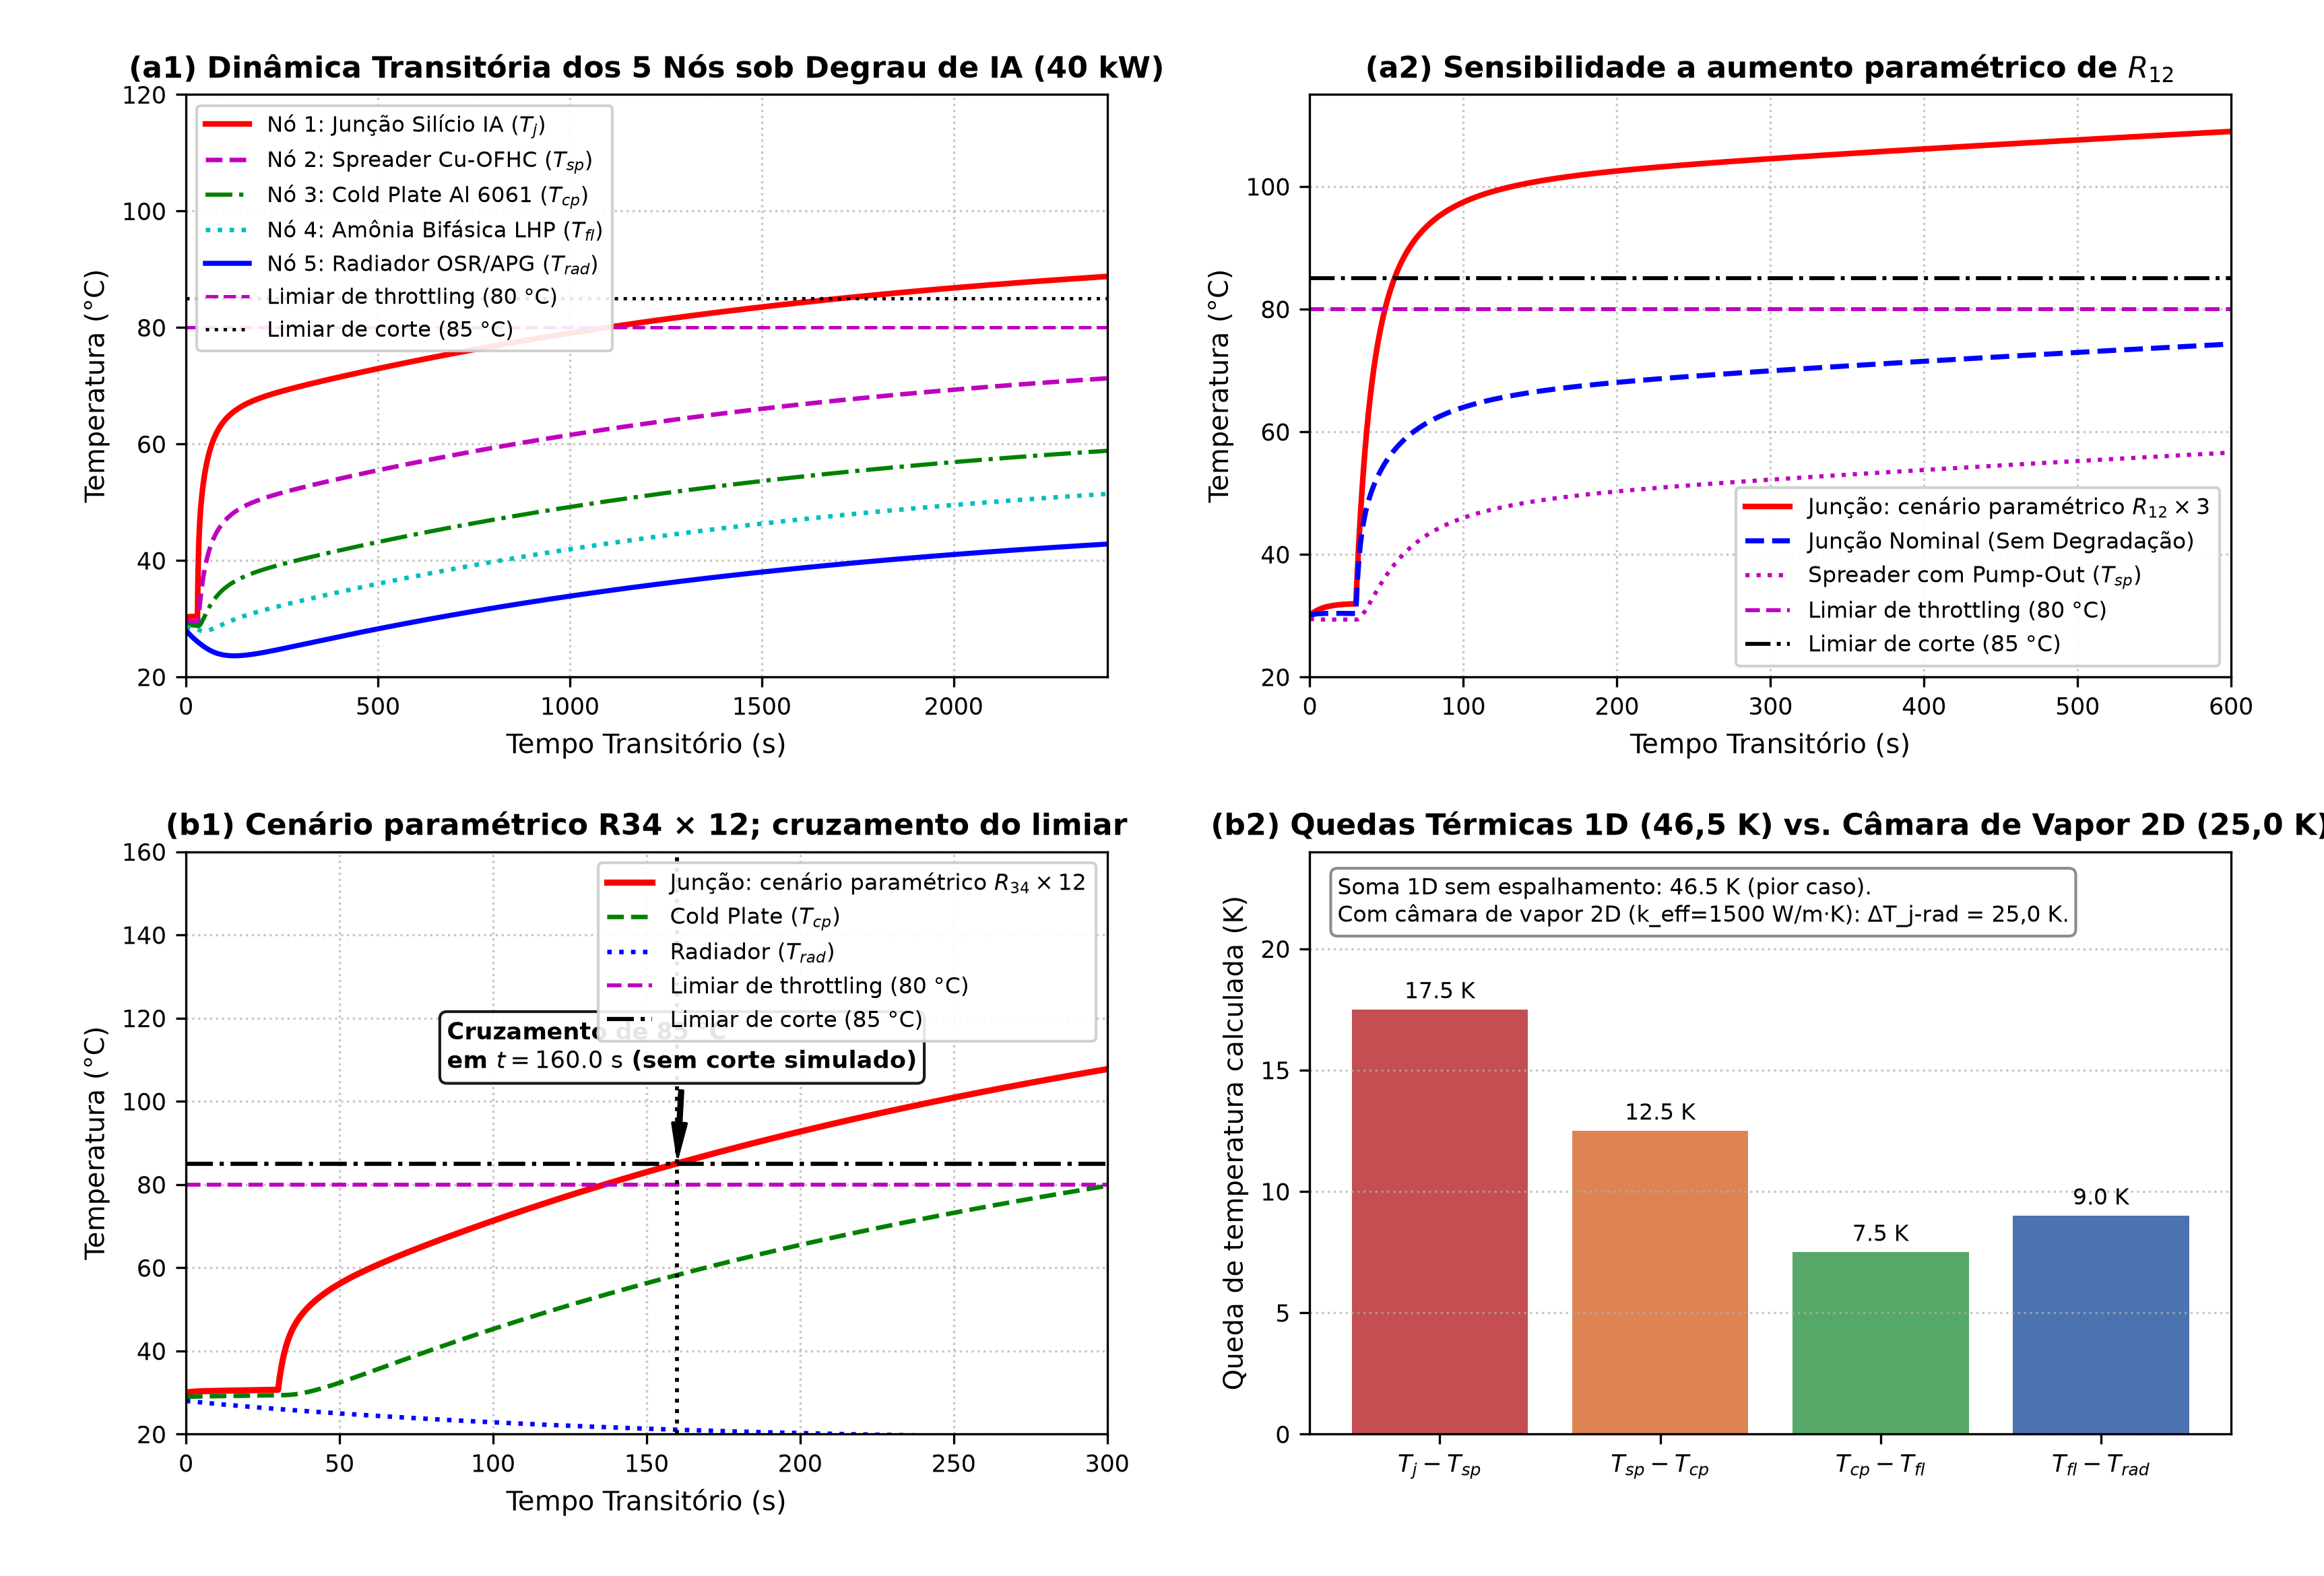
\includegraphics[width=0.82\textwidth]{figuras/figura_4_2_dinamica_rede_nodal_estresse.png}
    \caption{Simulação exploratória em malha aberta da rede nodal com parâmetros provisórios: (a1) degrau imposto de 2 para 40~kW em $t=30$~s; no caso nominal, $T_j$ cruza 80~$^\circ$C em 1256~s e 85~$^\circ$C em 2042{,}5~s, sem que o script aplique throttling ou corte; (a2) sensibilidade a $R_{12}\times3$, com cruzamentos calculados em 49~s e 55~s; (b1) sensibilidade a $R_{34}\times12$, com cruzamentos em 135~s e 157{,}5~s; (b2) contribuição de cada resistência para a queda calculada de 46{,}5~K a 40~kW, incompatível com os 25~K usados no balanço reduzido. Os multiplicadores não foram derivados de ensaios de falha, e a figura não é validação do LHP, do TIM ou do controlador.}
    \label{fig:dinamica_rede_nodal_estresse}
\end{figure}

A leitura da Figura~\ref{fig:dinamica_rede_nodal_estresse} deve permanecer restrita aos parâmetros inseridos no integrador explícito e ao horizonte simulado:
\begin{enumerate}[label=(\alph*)]
    \item \textbf{Caso nominal (Subpainel~a1):} Com o estado inicial imposto e o degrau de 40~kW em $t=30$~s, em $t=600$~s o integrador calcula $T_j=74{,}76^\circ$C, $T_{sp}=57{,}29^\circ$C, $T_{cp}=44{,}90^\circ$C, $T_{fl}=37{,}62^\circ$C e $T_{rad}=29{,}42^\circ$C. A resposta ainda é transitória. Na extensão de 2400~s, a malha aberta cruza 80~$^\circ$C em 1256~s e 85~$^\circ$C em 2042{,}5~s. Como nenhuma ação TEMS ou desligamento é aplicada, a continuação após esses cruzamentos é contrafactual e não demonstra operação segura;
    
    \item \textbf{Sensibilidade de $R_{12}$ (Subpainel~a2):} O multiplicador paramétrico $R_{12}\times3$ cruza 80~$^\circ$C em 49~s e 85~$^\circ$C em 55~s. Esses tempos resultam do integrador e das condições iniciais; não são tempos de falha de um TIM real nem incluem acionamento do controlador;
    
    \item \textbf{Sensibilidade de $R_{34}$ (Subpainel~b1):} O multiplicador $R_{34}\times12$ cruza 80~$^\circ$C em 135~s e 85~$^\circ$C em 157{,}5~s. O script não relaciona esse multiplicador à perda de vazão, ao limite capilar ou ao CHF, e não executa o corte de hardware;
    
    \item \textbf{Reconciliação das resistências (Subpainel~b2):} Para 40~kW atravessando a cadeia, as quedas nos quatro elementos somam 46{,}5~K. Isso não coincide com $\Delta T_{j-rad}=25$~K do modelo concentrado da Figura~\ref{fig:fluxos_orbitais_comparativos}; a diferença permanece aberta até que os parâmetros sejam obtidos para uma arquitetura definida.
\end{enumerate}

\subsection{Modelagem Radiativa e Dimensionamento Óptico do Radiador Espacial}
\label{sec:modelagem_radiador_espacial}

A rejeição térmica de centros de dados espaciais no vácuo apoia-se com exclusividade na radiação superficial para o espaço circundante. Para garantir a rigorosa homogeneidade dimensional e eliminar ambiguidades entre densidade de fluxo ($\text{W/m}^2$) e potência térmica ($\text{W}$), formula-se o balanço térmico radiativo superficial em termos da taxa líquida de calor rejeitado para o espaço ($Q_{net,rej}$, expresso estritamente em Watts):
\begin{equation}
    Q_{net,rej}(t) = Q_{emit}(t) - P_{abs,amb}(t) \quad \text{[W]}
    \label{eq:balanco_liquido_radiador_potencia}
\end{equation}
em que $Q_{emit}(t)$ é a potência térmica bruta emitida pela área ativa do radiador ($A_{rad}$) e $P_{abs,amb}(t)$ é a potência radiativa parasita total absorvida a partir das fontes ambientais externas (Sol, albedo e infravermelho terrestre).

A potência emitida no modelo reduzido de corpo cinzento difuso é calculada em relação ao fundo radiativo ($T_{space}$):
\begin{equation}
    Q_{emit}(t) = \varepsilon_{ir}(t) \cdot \sigma \cdot A_{rad} \cdot \eta_{fin} \cdot \left( T_{rad}^4(t) - T_{space}^4 \right) \quad \text{[W]}
    \label{eq:stefan_boltzmann_radiador_rigoroso}
\end{equation}
onde:
\begin{itemize}[leftmargin=*]
    \item $\sigma = 5{,}67037 \times 10^{-8}\text{ W/(m}^2\text{K}^4)$ é a constante fundamental de Stefan-Boltzmann;
    \item $\varepsilon_{ir}(t)$ é a emissividade hemisférica no infravermelho térmico ($\lambda \approx 4\text{ a }50\ \mu\text{m}$);
    \item $A_{rad}$ é a área superficial total de emissão radiativa livre (para painéis desdobráveis bifaciais com ambas as faces expostas ao espaço, $A_{rad} = 2 A_{painel}$);
    \item $\eta_{fin}$ é a eficiência média de aleta radiativa;
    \item $T_{rad}(t)$ é a temperatura média termodinâmica absoluta da superfície externa do radiador;
    \item $T_{space}=3{,}0\text{ K}$ é a temperatura de fundo usada no termo de emissão. A absorção de IR terrestre e albedo é contabilizada uma única vez em $P_{abs,amb}$, na Equação~(\ref{eq:potencia_parasita_absorvida}); portanto, não se inclui simultaneamente um sumidouro terrestre equivalente em $Q_{emit}$. Esta é uma aproximação de balanço concentrado: a emissão do radiador para o disco terrestre não é modelada como uma rede radiativa própria.
\end{itemize}

A potência ambiental parasita total absorvida ($P_{abs,amb}$) decompõe-se rigorosamente nas áreas projetadas e fatores de forma geométricos:
\begin{align}
    P_{abs,amb}(t) &= \underbrace{\alpha_s(t) \cdot A_{sol,proj}(t) \cdot G_{AM0} \cdot S(t)}_{\text{Absorção Solar Direta}} \nonumber \\
    &\quad + \underbrace{\alpha_s(t) \cdot A_{rad} \cdot F_{rad-E}(h, \phi) \cdot a_E \cdot G_{AM0} \cdot S(t) \cdot \max(0, \cos \theta_{sun,nadir})}_{\text{Absorção de Albedo Terrestre}} \nonumber \\
    &\quad + \underbrace{\varepsilon_{ir}(t) \cdot A_{rad} \cdot F_{rad-E}(h, \phi) \cdot q_{Earth}}_{\text{Absorção Infravermelha Terrestre}} \quad \text{[W]}
    \label{eq:potencia_parasita_absorvida}
\end{align}
onde $A_{sol,proj}(t) = A_{rad} \cdot \max(0, \, \hat{\mathbf{n}}_{rad} \cdot \hat{\mathbf{s}}(t))$ é a área efetiva projetada normal ao vetor solar. Na atitude nominal estática em órbita heliossíncrona *Dawn-Dusk*, a normal do radiador aponta permanentemente para o semiplano anti-solar ($\hat{\mathbf{n}}_{rad} \cdot \hat{\mathbf{s}} \le 0$), anulando $A_{sol,proj} = 0\text{ m}^2$ em regime nominal.

\subsubsection{Condução Bidimensional em Aletas de APG Anisotrópico e Eficiência \texorpdfstring{($\eta_{fin}$)}{(eta_fin)}}

O transporte de calor entre os tubos coletores do condensador bifásico de amônia e as extremidades emissoras do radiador depende da condução sólida bidimensional nas aletas. Diferentemente de metais isotrópicos homogêneos, adota-se uma estrutura avançada de \textbf{Grafite Pirolítico Encapsulado} (\textit{Annealed Pyrolytic Graphite} -- APG). O APG exibe condutividade térmica planar extraordinária no plano basal cristalográfico ($k_{xx} = k_{yy} = k_{in-plane} \ge 1500\text{ W/(m}\cdot\text{K)}$), mas baixa condutividade transversal através das lamelas de grafeno ($k_{zz} = k_{through-plane} \approx 10\text{ W/(m}\cdot\text{K)}$).

Para conferir rigidez estrutural e mitigar a fragilidade mecânica do grafite sob cargas de lançamento, o núcleo de APG de espessura $t_{APG} = 1{,}5\text{ mm}$ é encapsulado em facesheets estruturais de compósito de fibra de carbono de ultra-alto módulo K13D2U em matriz cianato-éster de espessura $t_c = 0{,}25\text{ mm}$ e condutividade $k_c = 600\text{ W/(m}\cdot\text{K)}$. A condutividade térmica efetiva no plano da aleta compósita sanduíche ($k_{eff}$) é calculada pela média ponderada das camadas paralelas:
\begin{align}
    k_{eff} &= \frac{k_{in-plane} t_{APG} + 2 k_c t_c}{t_{APG} + 2 t_c} \nonumber \\
    &= \frac{1500 \cdot 1{,}5 + 2 \cdot 600 \cdot 0{,}25}{2{,}0} = 1275{,}0\text{ W/(m}\cdot\text{K)} \quad \text{[VERIFICÁVEL]}
    \label{eq:condutividade_efetiva_apg}
\end{align}

Considerando uma aleta retangular de comprimento livre $L_{fin} = 75\text{ mm}$ entre tubos condutores de condensação espaçados de $2 L_{fin} = 150\text{ mm}$, a equação diferencial de condução de calor unidimensional em regime permanente ao longo da coordenada longitudinal $x$ da aleta, com emissão radiativa simétrica em ambas as faces para o fundo $T_{space}$, é governada por:
\begin{equation}
    k_{eff} t_{fin} \frac{d^2 T(x)}{dx^2} = 2 \varepsilon_{ir} \sigma \left( T^4(x) - T_{space}^4 \right), \quad 0 \le x \le L_{fin}
    \label{eq:equacao_aleta_nao_linear_exata}
\end{equation}
sujeita às condições de contorno de Dirichlet na raiz condutora e de Neumann (adiabática) na ponta de simetria:
\begin{equation}
    T(0) = T_{root} = 45{,}0^\circ\text{C} = 318{,}15\text{ K}, \qquad \left. \frac{dT}{dx} \right|_{x = L_{fin}} = 0
    \label{eq:condicoes_contorno_aleta}
\end{equation}

Como o gradiente térmico ao longo da aleta de APG é pequeno em virtude de sua elevadíssima condutividade ($k_{eff} = 1275\text{ W/(m}\cdot\text{K)}$), lineariza-se a troca radiativa quártica através da expansão em série de Taylor em torno da temperatura média da raiz ($T_{root}$):
\begin{equation}
    T^4(x)-T_{space}^4 = (T(x)-T_{space})(T(x)+T_{space})(T^2(x)+T_{space}^2) \approx h_{rad}(T(x)-T_{space}), \quad h_{rad}=\varepsilon_{ir}\sigma(T_{root}+T_{space})(T_{root}^2+T_{space}^2)\approx1{,}512\text{ W/(m}^2\text{K)}
    \label{eq:coeficiente_linearizado_hrad}
\end{equation}
A integração analítica fechada da equação diferencial linearizada resulta no perfil hiperbólico de temperatura $\theta(x) = \theta_{root} \cosh[m (L_{fin} - x)] / \cosh(m L_{fin})$, definindo a eficiência de aleta radiativa ($\eta_{fin}$):
\begin{equation}
    \eta_{fin,ideal} = \frac{\tanh(m L_{fin})}{m L_{fin}}, \qquad m = \sqrt{\frac{2 h_{rad}}{k_{eff} t_{fin}}} = \sqrt{\frac{2 \cdot 1{,}512}{1275 \cdot 0{,}0020}} \approx 1{,}089\text{ m}^{-1}
    \label{eq:eficiencia_aleta_apg_rigorosa}
\end{equation}
Para $L_{fin} = 0{,}075\text{ m}$, tem-se $m L_{fin} = 0{,}1683$, resultando em uma eficiência excepcional de:
\begin{equation}
    \eta_{fin,ideal} = \frac{\tanh(0{,}0817)}{0{,}0817} \approx \mathbf{0{,}9978} \quad (> 99\%)
\end{equation}
O valor $\eta_{fin}=0{,}945$ empregado no script é uma premissa de projeto [PROVISÓRIA]; não há modelo de contato ou ensaio no repositório que demonstre que essa margem represente perdas reais. A eficiência ideal calculada da aleta e o fator efetivo usado no balanço devem, portanto, permanecer identificados separadamente.

\subsubsection{Modelo Dinâmico de Degradação Óptica Temporal (BOL para EOL em 10 Anos)}

As propriedades termo-ópticas dos revestimentos externos degradam-se de forma não linear ao longo dos 10 anos de vida útil de projeto, em decorrência do escurecimento fotoquímico sob radiação ultravioleta do vácuo cósmico (\textit{vacuum UV solar browning}), impactos de oxigênio atômico (AO) e deposição de filmes moleculares desgaseificados da espaçonave (\textit{molecular contamination outgassing}). Rejeita-se a soma estática de constantes arbitrárias e adota-se o modelo físico de evolução temporal por saturação exponencial, recomendado pela norma ECSS-E-HB-31-01 Parte 6:
\begin{equation}
    \alpha_s(t) = \alpha_{s,BOL} + \left( \alpha_{s,EOL} - \alpha_{s,BOL} \right) \left[ 1 - \exp\left( -\frac{t}{\tau_{deg}} \right) \right]
    \label{eq:lei_degradacao_optica_temporal}
\end{equation}
onde:
\begin{itemize}[leftmargin=*]
    \item Para os **Espelhos Ópticos Solares de Quartzo/Prata (OSR)** aplicados sobre os radiadores térmicos: $\alpha_{s,BOL} = 0{,}08$, saturando em $\alpha_{s,EOL} = 0{,}14$ em 10 anos, com constante de tempo de saturação por radiação UV $\tau_{deg,OSR} = 3{,}2\text{ anos}$. A emissividade térmica no infravermelho mantém-se praticamente inalterada e estável em $\varepsilon_{ir} = 0{,}88 \pm 0{,}01$, pois o quartzo fundido é inerte à erosão por AO;
    \item Para a **Tinta Branca Cerâmica de Silicato (AZ-93)** empregada na carcaça estrutural externa: $\alpha_{s,BOL} = 0{,}15$, degradando para $\alpha_{s,EOL} = 0{,}26$, com constante de tempo $\tau_{deg,AZ} = 2{,}1\text{ anos}$ e $\varepsilon_{ir} = 0{,}91 \rightarrow 0{,}89$.
\end{itemize}

O impacto térmico direto dessa degradação sobre o radiador na órbita heliossíncrona reside no aumento de $+75\%$ na absortividade solar ($\Delta \alpha_s = +0{,}06$). Como a atitude nominal é anti-solar, a absorção de albedo terrestre residual (Eq.~\ref{eq:potencia_parasita_absorvida}) cresce ligeiramente de $2{,}17\text{ W/m}^2$ para $3{,}80\text{ W/m}^2$. A elevação efetiva de temperatura de equilíbrio da carcaça do satélite ao longo da década situa-se em $\Delta T_{eq} \approx +3{,}8\text{ K}$ na atitude nominal, e alcança $+12\text{ a }+16\text{ K}$ apenas se houver exposição solar direta de faces estruturais revestidas com AZ-93.

\subsubsection{Sensibilidade Térmica a Desvios de Atitude e Análise de Margem Operacional}

Para substituir noções imprecisas de ``saturação anti-solar'', modela-se rigorosamente o impacto térmico de um \textbf{desvio angular de atitude} ($\delta \theta_{att}$) do sistema de controle de atitude (ADCS) em relação ao vetor anti-solar ideal. Se a plataforma sofrer uma perturbação de guinada ou arfagem de magnitude $\delta \theta_{att}$, a face do radiador deixa de estar na sombra do corpo principal e passa a interceptar radiação solar direta com área projetada $A_{sol,proj} = A_{rad} \sin |\delta \theta_{att}|$.

A densidade de fluxo solar direto incidente absorvido passa a ser:
\begin{equation}
    q_{sol,abs,pert}(t) = \alpha_{s}(t) \cdot G_{AM0} \cdot \sin |\delta \theta_{att}|
    \label{eq:fluxo_solar_perturba_atitude}
\end{equation}
Para um desvio angular $|\delta \theta_{att}|$ sob as propriedades EOL assumidas no script ($\alpha_{s,EOL}=0{,}24$):
\begin{equation}
    q_{sol,abs,pert} = \alpha_{s,EOL} G_{AM0} \sin(|\delta\theta_{att}|)
\end{equation}
Para $A_{rad}=88{,}6\text{ m}^2$, $Q_{int}=41{,}984\text{ kW}$, $\varepsilon_{ir,EOL}=0{,}82$, $\eta_{fin}=0{,}945$ e o fluxo ambiental médio SSO calculado de $52{,}48\text{ W/m}^2$, o modelo prevê, já em $\delta\theta=0^\circ$, $T_{rad}=57{,}68^\circ\text{C}$ e $T_j=82{,}68^\circ\text{C}$ usando $\Delta T_{j-rad}=25\text{ K}$ [PROVISÓRIO]. Isso supera o teto de $55^\circ\text{C}$ do radiador e a meta de throttling de $80^\circ\text{C}$. O limiar de $85^\circ\text{C}$ é alcançado pelo modelo perto de $2{,}62^\circ$ de desvio. A área de sensibilidade de $92{,}0\text{ m}^2$ resulta em $T_{rad}=54{,}89^\circ\text{C}$ e $T_j=79{,}89^\circ\text{C}$ nas mesmas condições; ela não substitui o dimensionamento de EOL com perdas e incertezas fechadas.

A Tabela~\ref{tab:dimensionamento_radiador_comparativo} registra os resultados reproduzíveis do modelo reduzido. O script calcula fluxos para SSO e LEO; embora calcule o período orbital GEO, não calcula para GEO a sombra, os fluxos absorvidos ou o balanço térmico. Os valores de área abaixo são estimativas condicionais em equilíbrio, não qualificação de projeto.

\begin{table}[!ht]
\centering
\small
\renewcommand{\arraystretch}{0.85}
\caption{Resultados do balanço radiativo EOL adotado para SSO e LEO. Os valores GEO não são calculados pelo script atual.}
\label{tab:dimensionamento_radiador_comparativo}
\resizebox{0.95\textwidth}{!}{%
\begin{tabular}{lcccc}
\hline
\textbf{Parâmetro de Dimensionamento Radiativo} & \textbf{SSO Dawn-Dusk (700 km)} & \textbf{LEO Convencional (500 km)} & \textbf{GEO (35.786 km)} & \textbf{Classificação Epistêmica} \\ \hline
Potência térmica de entrada usada ($Q_{int}$) & $41{,}984\text{ kW}$ & $41{,}984\text{ kW}$ & -- & \textbf{[ENTRADA DO SCRIPT]} Rastrear com o balanço elétrico do nó \\
Fator de visão radiador--Terra ($F_{rad-E}$) & $0{,}2328$ & $0{,}4473$ & -- & \textbf{[CALCULADO]} GEO ainda não avaliado radiativamente \\
Fluxo parasita médio ($q_{parasita}$) & $52{,}48\text{ W/m}^2$ & $97{,}95\text{ W/m}^2$ (pico $194{,}88$) & -- & \textbf{[CALCULADO]} Média orbital do script; LEO é transiente \\
Emissão no limite $T_{rad}=55^\circ$C & $509{,}50\text{ W/m}^2$ & $509{,}50\text{ W/m}^2$ & $509{,}50\text{ W/m}^2$ & \textbf{[CALCULADO]} $\varepsilon_{EOL}\sigma\eta_{fin}(T_{rad}^4-T_{space}^4)$ \\
Capacidade líquida em $55^\circ$C ($q_{net,rej}$) & $457{,}02\text{ W/m}^2$ & $411{,}55\text{ W/m}^2$ (média) & -- & \textbf{[CALCULADO]} Não inclui margem de incerteza \\
Área de equilíbrio requerida a $55^\circ$C & $91{,}86\text{ m}^2$ & $102{,}02\text{ m}^2$ (média) & -- & \textbf{[CALCULADO]} $Q_{int}/q_{net,rej}$; LEO não é sizing dinâmico \\
Área adotada no caso SSO & $88{,}6\text{ m}^2$ & -- & -- & \textbf{[PREMISSA DE PROJETO]} Resultado: $T_{rad}=57{,}68^\circ$C, $T_j=82{,}68^\circ$C \\ \hline
\end{tabular}%
}
\end{table}

A avaliação atual compara fluxos orbitais em SSO e LEO. Para o caso EOL modelado, o fluxo parasita médio é $52{,}48\text{ W/m}^2$ em SSO e $97{,}95\text{ W/m}^2$ em LEO, com pico orbital LEO de $194{,}88\text{ W/m}^2$. Esses valores dependem da geometria e das propriedades termo-ópticas assumidas. O script não calcula balanço radiativo GEO; portanto, não se apresenta comparação térmica de três órbitas nem se afirma dimensionamento GEO.

A síntese dos fluxos ambientais SSO/LEO e da sensibilidade do equilíbrio térmico ao erro de atitude é apresentada na Figura~\ref{fig:fluxos_orbitais_comparativos}.

\begin{figure}[htbp]
    \centering
    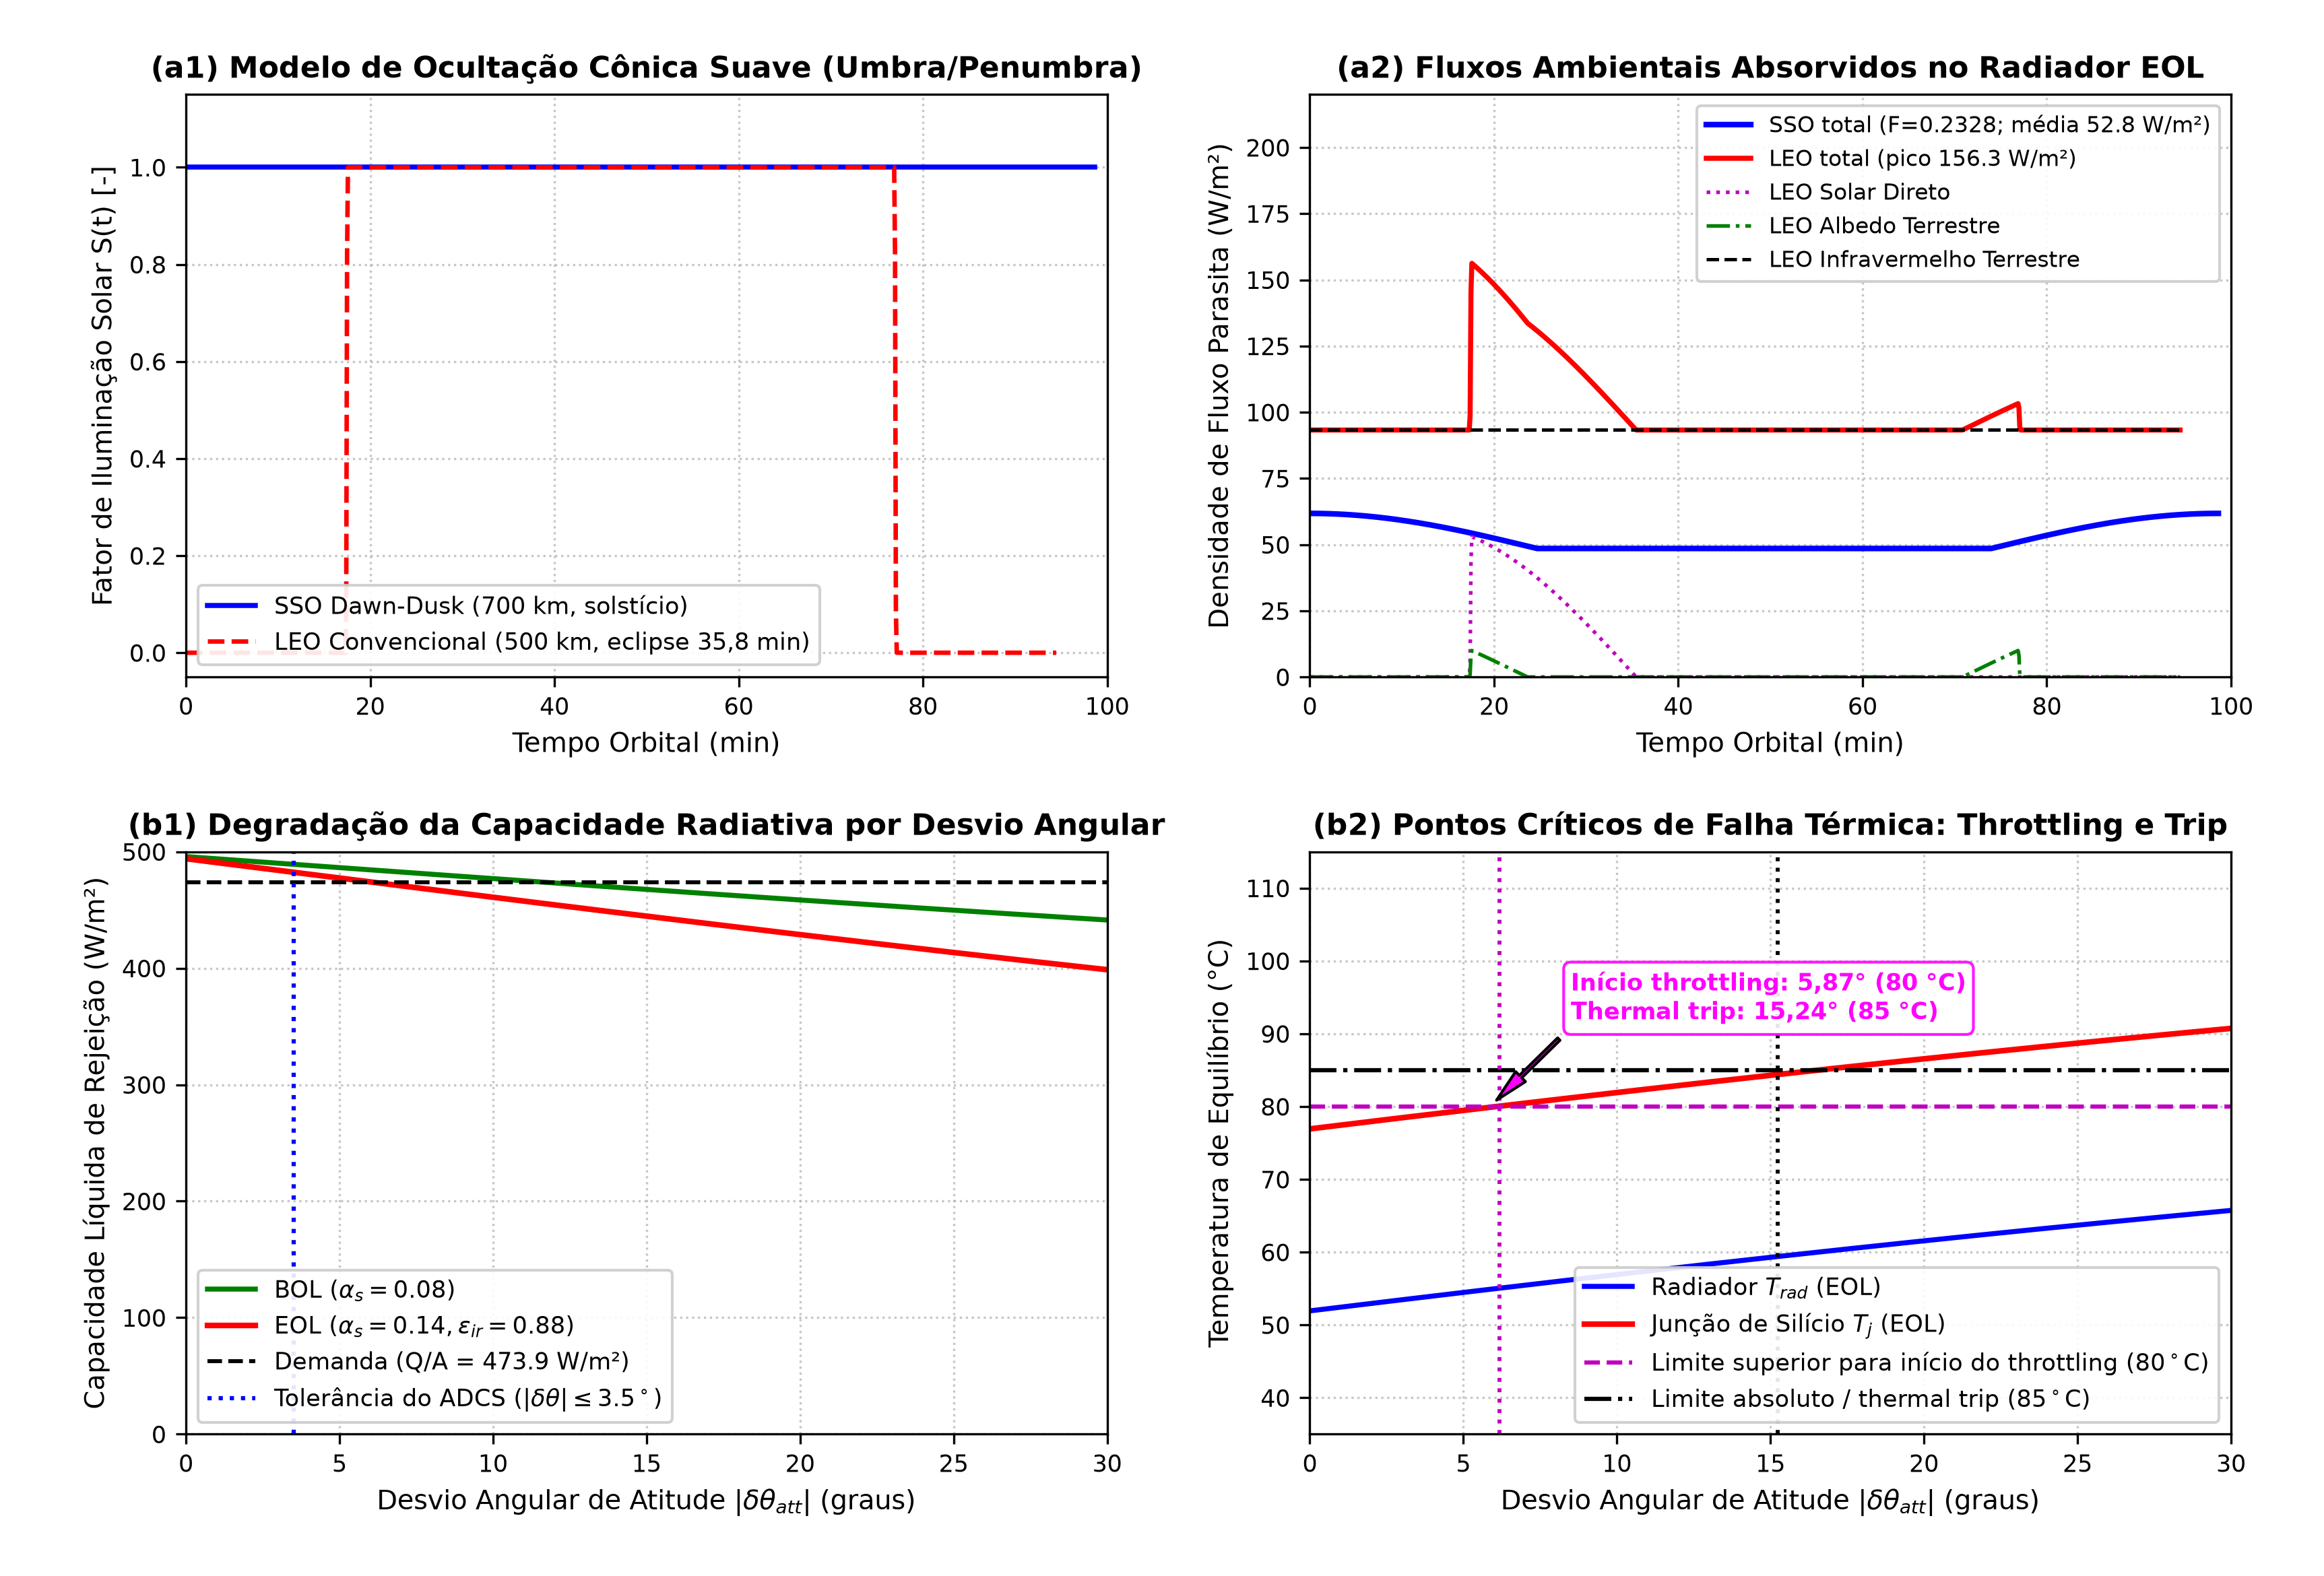
\includegraphics[width=0.82\textwidth]{figuras/figura_4_1_fluxos_orbitais_comparativos.png}
    \caption{Modelo radiativo reduzido para SSO e LEO: (a1) fator de iluminação em uma revolução, com eclipse LEO; (a2) fluxos ambientais absorvidos usando propriedades EOL assumidas; (b1) capacidade líquida de rejeição em função do erro de atitude, comparada à demanda térmica; (b2) temperaturas de equilíbrio do radiador e da junção, com o limite de início de throttling em $80^\circ$C e o limite absoluto em $85^\circ$C. O SSO nominal já excede $80^\circ$C no caso EOL calculado. GEO não é simulado nesta figura.}
    \label{fig:fluxos_orbitais_comparativos}
\end{figure}

A decomposição dos quatro subpainéis da Figura~\ref{fig:fluxos_orbitais_comparativos} evidencia:
\begin{enumerate}[label=(\alph*)]
    \item \textbf{Iluminação orbital (Subpainel~a1):} O cenário LEO de 500~km e $\beta=20^\circ$ produz eclipse de cerca de $35{,}8$~min por revolução no modelo cônico. O SSO a $700$~km e $\beta=85^\circ$ não apresenta eclipse no ciclo nominal representado; a figura não calcula a evolução sazonal anual de $\beta$;
    
    \item \textbf{Fluxos ambientais (Subpainel~a2):} Para SSO, $F_{rad-E}=0{,}2328$, o albedo médio absorvido calculado é $7{,}25\text{ W/m}^2$ e o IR terrestre absorvido é $45{,}23\text{ W/m}^2$, totalizando $52{,}48\text{ W/m}^2$. Para LEO, o script calcula média de $97{,}95\text{ W/m}^2$ e pico de $194{,}88\text{ W/m}^2$. São resultados de uma órbita e das propriedades EOL provisórias, não uma caracterização anual;
    
    \item \textbf{Margem térmica e erro de atitude (Subpainéis~b1/b2):} Com $A_{rad}=88{,}6\text{ m}^2$, a demanda $Q_{int}/A_{rad}=473{,}86\text{ W/m}^2$ já excede a capacidade líquida do caso SSO em $55^\circ$C ($457{,}02\text{ W/m}^2$). O equilíbrio nominal calculado é $T_{rad}=57{,}68^\circ$C e $T_j=82{,}68^\circ$C; assim, a condição já requer throttling antes de qualquer erro de atitude. O limite de $85^\circ$C é alcançado perto de $2{,}62^\circ$ de desvio no modelo; o limiar de trip é $85^\circ$C, não $105^\circ$C;
    
    \item \textbf{Área condicional e escopo GEO:} A $55^\circ$C, o modelo requer $91{,}86\text{ m}^2$ em SSO e $102{,}02\text{ m}^2$ em LEO se usado o fluxo LEO médio; o cálculo não incorpora a resposta térmica transiente nem margem de incerteza. A área SSO adotada de $88{,}6\text{ m}^2$ é insuficiente para a carga térmica usada. O código atual não calcula os fluxos ou a área GEO.
\end{enumerate}

\subsection{Dinâmica de Co-Design Eletrotérmico de Chips de IA e Condição Analítica de Instabilidade}
\label{sec:co_design_eletrotermico_runaway}

A modelagem térmica no nível de silício exige a integração acoplada entre o comportamento elétrico dos circuitos semicondutores e a dinâmica de transferência de calor. Em nós litográficos avançados com transistores FinFET e Gate-All-Around (GAA) sub-7~nm, a elevação da temperatura de junção ($T_j$) induz o aumento exponencial das correntes térmicas de fuga quântica e termoiônica. Esse acoplamento eletrotérmico bidirecional estabelece uma retroalimentação não linear que, na ausência de capacidade adequada de extração térmica, pode deflagrar a divergência térmica descontrolada (\textit{thermal runaway}).

\subsubsection{Fronteira de Potência no Nó e Decomposição da Dissipação}

Para evitar duplicidade com os modelos do Capítulo~\ref{sec:arquitetura_barramento_balanco}, a potência entregue ao nó ($P_{node}$) decompõe-se em:
\begin{equation}
    P_{node}(t) = \underbrace{P_{core}(t) + P_{mem}(t)}_{P_{chip}(t)} + P_{VRM}(t) + P_{interconnect}(t) \quad \text{[W]}
    \label{eq:decomposicao_potencia_no}
\end{equation}
sendo $P_{chip}$ a dissipação nos aceleradores de IA (núcleos e memórias HBM3e em interposer CoWoS), $P_{VRM} \approx 2{,}3\text{ kW}$ as perdas dos conversores GaN PoL ($\eta_{PoL} \approx 94{,}5\%$), e $P_{interconnect} \approx 650\text{ W}$ a potência de barramentos PCIe 5.0/CXL e roteadores ópticos.

A potência do acelerador neural decompõe-se na componente dinâmica e na fuga sublimiar:
\begin{equation}
    P_{chip}(V_{core}, f_{clk}, T_j) = P_{dyn}(V_{core}, f_{clk}) + P_{leak}(T_j, V_{core}) \quad \text{[W]}
    \label{eq:potencia_total_chip_rigorosa}
\end{equation}
com potência dinâmica calibrada por $P_{dyn} = (\alpha_{act} C_{eff}) V_{core}^2 f_{clk}$, em que $(\alpha_{act} C_{eff})_{inf} \approx 171{,}0\text{ nF}$ para inferência e $334{,}4\text{ nF}$ para treinamento denso, operando em $V_{core} \in [0{,}65, 1{,}05]\text{ V}$ e $f_{clk} \in [1{,}0, 1{,}8]\text{ GHz}$.

\subsubsection{Modelo de Corrente de Fuga e Estabilidade Térmica (Thermal Runaway)}

A corrente de fuga sublimiar é modulada termicamente por emissão termoiônica e tunelamento quântico (formulação BSIM detalhada no Apêndice~B.7). Para processamento em tempo real, adota-se a formulação empírica calibrada:
\begin{equation}
    P_{leak}(T_j, V_{core}) = P_{leak,ref}(V_{core}) \cdot \exp\left[ \beta_T \left( T_j - T_{ref} \right) \right] \quad \text{[W]}
    \label{eq:potencia_fuga_calibrada_local}
\end{equation}
com $P_{leak,ref}(V_{core}) = I_{leak,ref} V_{core} (V_{core}/V_{core,nom})^2$, sendo $\beta_T = 0{,}0285\text{ K}^{-1}$ [PROVISÓRIO].

A estabilidade de equilíbrio de primeira ordem ($P_{chip}(T_j^*) = \dot{Q}_{out}(T_j^*)$) sob extração $\dot{Q}_{out} = (T_j - T_{sink})/R_{th,j-sink}$ com dependência de transporte capilar $R_{th,j-sink}(Q) = R_{th,0} [1 + (Q/Q_{max,cap})^4]$ impõe a condição estrita de Lyapunov para amortecimento:
\begin{equation}
    \left. \frac{\partial P_{chip}}{\partial T_j} \right|_{T_j^*} < \left. \frac{d\dot{Q}_{out}}{dT_j} \right|_{T_j^*} = \frac{1/R_{th}}{1+\frac{(T_j^*-T_{sink})}{R_{th}^{2}}\left.\frac{dR_{th}}{d\dot Q_{out}}\right|_*} \quad \text{[DEPENDENTE DO MODELO]}
    \label{eq:criterio_estabilidade_box}
\end{equation}
Para as condições nominais ($T_j^* = 70^\circ\text{C}$, $V_{core} = 0{,}85\text{ V}$, $P_{leak} \approx 3{,}6\text{ kW}$), o gradiente de fuga é $\partial P_{leak}/\partial T_j = \beta_T P_{leak} \approx 102{,}6\text{ W/K}$, muito inferior à condutância nominal agregada de $860{,}2\text{ W/K}$ (80 dies em paralelo), garantindo estabilidade. Sob falha severa ($R_{th}$ elevado para $\ge 0{,}35\text{ K/W}$ por degradação de TIM ou dry-out), a condutância cai para $\le 228{,}5\text{ W/K}$. Caso $T_j$ atinja $95^\circ\text{C}$ ($P_{leak} \approx 7{,}4\text{ kW}$), o gradiente sobe para $210{,}9\text{ W/K}$, aproximando-se do limiar de bifurcação de \textit{thermal runaway}.

A violação do envelope de temperatura deflagra as proteções: (a) \textit{thermal throttling} gradual antes de $80^\circ\text{C}$ (reduzindo $f_{clk}$ de $1{,}8$ para $1{,}0\text{ GHz}$); (b) \textit{thermal trip} rígido em $T_{crit} = 85{,}0^\circ\text{C}$ para modo seguro. A Figura~\ref{fig:estabilidade_runaway_lhp} ilustra o crescimento exponencial da fuga, a bifurcação de runaway sob tensão turbo ($1{,}05\text{ V}$) e o mapa de estabilidade no plano $V_{core} \times R_{th,crit}$.

\begin{figure}[htbp]
    \centering
    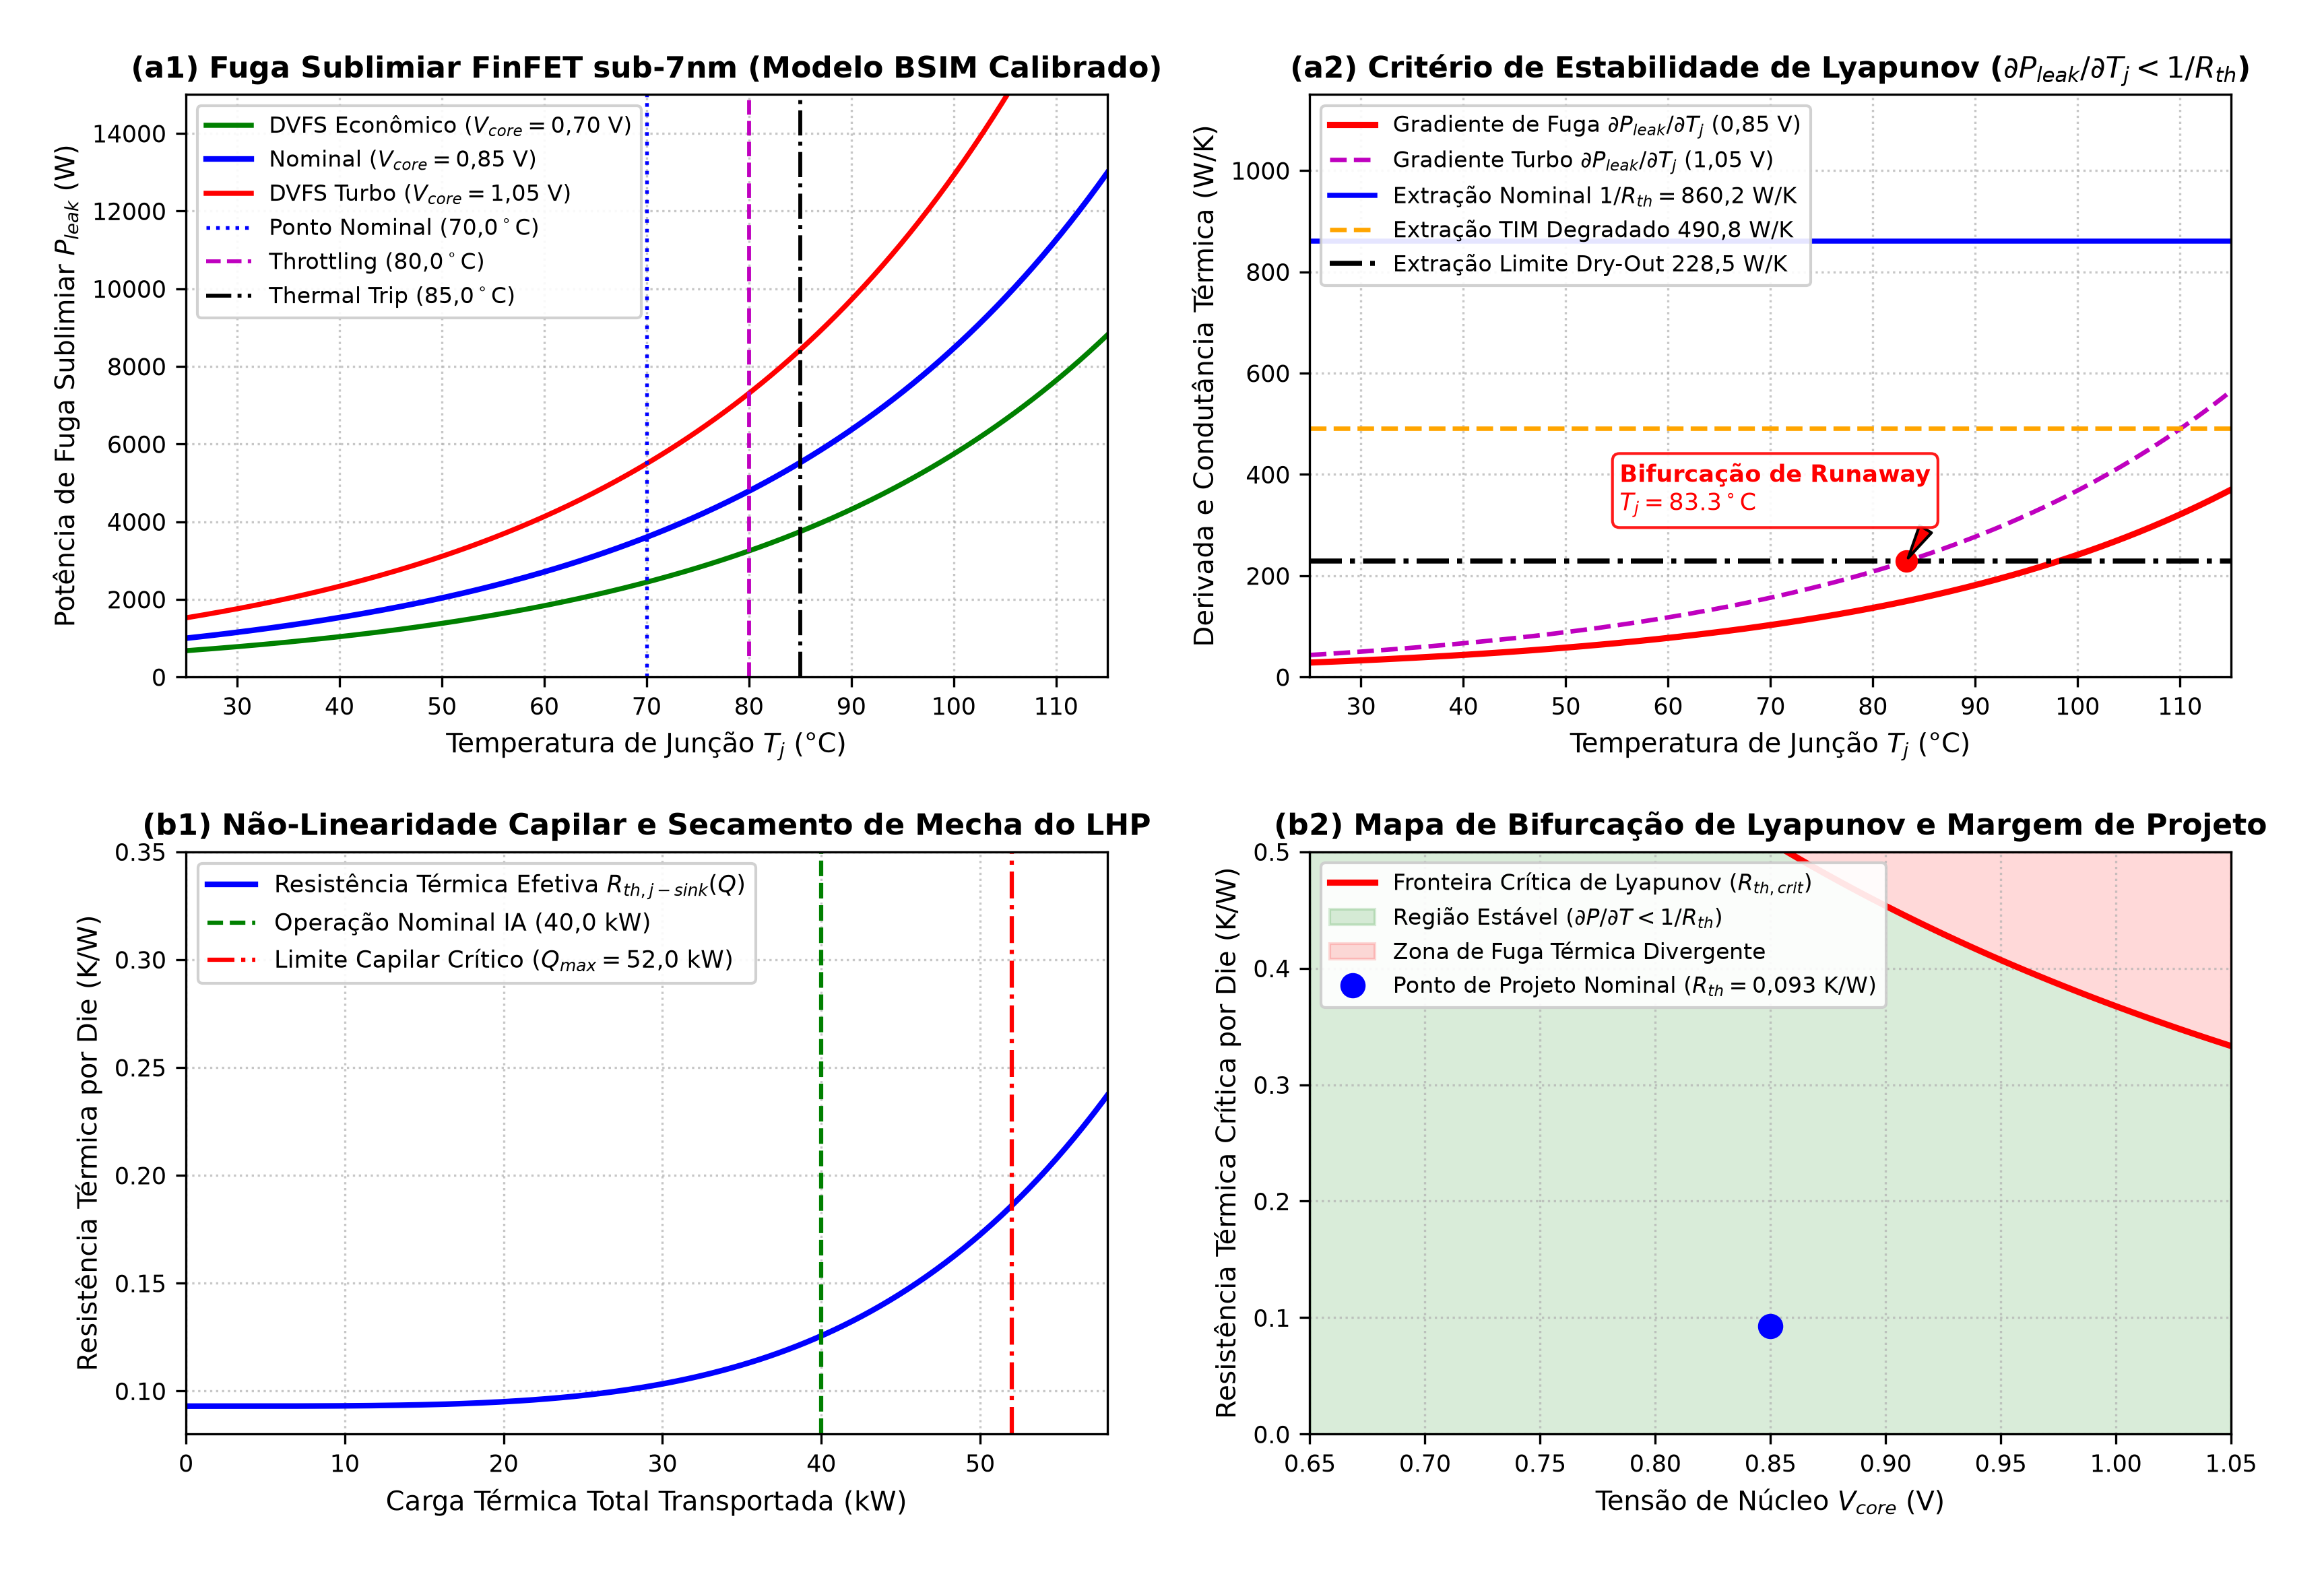
\includegraphics[width=0.82\textwidth]{figuras/figura_4_3_estabilidade_runaway_lhp.png}
    \caption{Co-design eletrotérmico e estabilidade de Lyapunov: (a1) fuga sublimiar calculada por modelo BSIM em função de $T_j$; (a2) critério de Lyapunov identificando bifurcação de runaway a $83{,}4^\circ\text{C}$ sob tensão turbo ($1{,}05\text{ V}$) e extração WCA; (b1) não linearidade da resistência do LHP governada pela aproximação quártica a $Q_{max} = 52{,}0\text{ kW}$; (b2) mapa de bifurcação no plano $V_{core} \times R_{th,crit}$, confirmando que o ponto nominal opera no interior da região estável.}
    \label{fig:estabilidade_runaway_lhp}
\end{figure}

\subsection{Sistema de Gerenciamento Térmico-Energético Ativo (TEMS)}
\label{sec:tems_arquitetura_controle}

Para prevenir que o sistema atinja limiares críticos de instabilidade térmica, minimizar as oscilações mecânicas de fadiga cíclica nas soldas e otimizar dinamicamente a entrega de processamento neural frente à geração solar orbitária e à carga da bateria, desenvolve-se a arquitetura de controle hierárquico em duas camadas do \textbf{Sistema de Gerenciamento Térmico-Energético Ativo} (\textit{Thermal and Energy Management System} -- TEMS).

\subsubsection{Classificação Epistêmica dos Limiares Operacionais de Projeto}

Para eliminar arbitrariedades de parametrização e fornecer rastreabilidade física de engenharia, a Tabela~\ref{tab:classificacao_limiares_tems} cataloga os limiares de controle, segurança e atuação do TEMS sob rigorosa classificação epistêmica.

\begin{table}[!ht]
\centering
\small
\renewcommand{\arraystretch}{0.85}
\caption{Classificação epistêmica e justificativa dos limiares operacionais do TEMS.}
\label{tab:classificacao_limiares_tems}
\resizebox{0.95\textwidth}{!}{%
\begin{tabular}{lcccc}
\hline
\textbf{Limiar / Parâmetro Operacional} & \textbf{Símbolo} & \textbf{Valor de Projeto} & \textbf{Classificação} & \textbf{Justificativa Física / Referência de Norma} \\ \hline
Temperatura Alvo em Regime Normal & $T_{target}$ & $75{,}0^\circ\text{C}$ ($348{,}15\text{ K}$) & \textbf{[REQUISITO DE PROJETO]} & Limite informado para operação normal \\
Limite para Início de Throttling & $T_{thr}<80^\circ\text{C}$ & Antes de $80^\circ\text{C}$ & \textbf{[REQUISITO DE PROJETO]} & Setpoint numérico ainda não definido \\
Temperatura de Corte para Modo Seguro (Thermal Trip) & $T_{crit}$ & $85{,}0^\circ\text{C}$ ($358{,}15\text{ K}$) & \textbf{[REQUISITO DE PROJETO]} & Limite definido para este estudo; não é alegação de limite JEDEC \\
Temperatura Máxima da Bateria BESS & $T_{bat,max}$ & $+35{,}0^\circ\text{C}$ ($308{,}15\text{ K}$) & \textbf{[REQUISITO DE PROJETO]} & Limite definido para este estudo \\
Temperatura Mínima da Bateria BESS & $T_{bat,min}$ & $+10{,}0^\circ\text{C}$ ($283{,}15\text{ K}$) & \textbf{[REQUISITO DE PROJETO]} & Limite definido para este estudo \\
Estado de Carga Mínimo & $SoC_{min}$ & $20{,}0\%$ & \textbf{[REQUISITO DE PROJETO]} & Equivale a $DoD\le80\%$ sob a mesma referência energética \\
Taxa Máxima de Variação de Frequência & $\Delta f_{slew,max}$ & $100{,}0\text{ MHz/s}$ & \textbf{[PROVISÓRIO]} & Limita choque térmico nas esferas de solda BGA \\
Temperatura Máxima do Radiador & $T_{rad,max}$ & $55{,}0^\circ\text{C}$ & \textbf{[REQUISITO DE PROJETO]} & Limite informado para o radiador \\
Banda de Histerese Térmica Anti-Chattering & $\Delta T_{hyst}$ & $3{,}0^\circ\text{C}$ & \textbf{[PROVISÓRIO]} & Amortece comutações espúrias de alta frequência \\ \hline
\end{tabular}%
}
\end{table}

\subsubsection{Camada Rápida Descentralizada: DVFS em Malha Fechada}

A camada rápida atua em nível de die semicondutor e conversores GaN PoL de ponto de carga com período de amostragem de controle sub-milissegundo ($\Delta t_{fast} \le 1{,}0\text{ ms}$). O seu objetivo primário é conter excursões térmicas de alta frequência provocadas por degraus de ativação de tensores lógicos.

A lei de atuação do DVFS modula o vetor de ponto operacional $u_{fast}[k] = [f_{clk}[k], V_{core}[k]]^T$ a partir da leitura filtrada dos diodos térmicos internos do die ($T_j$), seguindo a relação de mapeamento de tensão-frequência do fabricante ($V_{core} = V_{core,min} + \lambda_{DVFS} (f_{clk} - f_{clk,min})$). Para evitar instabilidades de ciclo limite e chaveamento espúrio (\textit{chattering}), implementa-se uma banda de histerese finita com dois limiares desacoplados:
\begin{equation}
    f_{clk}[k] = 
    \begin{cases}
        \max\left( f_{clk,min}, \, f_{clk}[k-1] - \Delta f_{step} \right), & \text{se } T_j[k] \ge T_{thr}, \quad T_{thr}<80^\circ\text{C} \\[0.2cm]
        \min\left( f_{clk,max}, \, f_{clk}[k-1] + \Delta f_{step} \right), & \text{se } T_j[k] \le T_{thr} - \Delta T_{hyst} \\[0.2cm]
        f_{clk}[k-1], & \text{se } T_{thr} - \Delta T_{hyst} < T_j[k] < T_{thr}
    \end{cases}
    \label{eq:dvfs_histerese_antichattering}
\end{equation}
em que o passo discreto de modulação de frequência é restrito pelo limitador de taxa (\textit{slew rate limiter}) para mitigar fadiga por choque mecânico nas soldas:
\begin{equation}
    \Delta f_{step} \le \Delta f_{slew,max} \cdot \Delta t_{fast} = 100\text{ MHz/s} \cdot 10^{-3}\text{ s} = 100\text{ kHz por ciclo}
\end{equation}

A resposta do DVFS não acarreta a paralisação abrupta ou colapso a zero do processamento, mas sim uma \textbf{redução temporária controlada de frequência} (reduzindo a dissipação dinâmica proporcionalmente a $f_{clk}$ e quadraticamente com $V_{core}$), preservando a integridade física e mantendo a vazão computacional no maior patamar compatível com a capacidade instantânea de resfriamento.

\subsubsection{Camada Lenta Supervisória Preditiva: Formulação NMPC com Consciência Orbital}

A camada supervisória do TEMS opera a uma taxa de amostragem de $\Delta t_{ctrl} = 3{,}0\text{ s}$, formulando o problema de controle sob a metodologia de \textbf{Controle Preditivo Baseado em Modelo Não Linear} (\textit{Nonlinear Model Predictive Control} -- NMPC) com horizonte de predição de $N_p = 20$ passos ($60\text{ segundos}$ à frente) e horizonte de controle $N_u = 10$ passos.

No regime normal, o critério de sucesso é $T_j\le75^\circ\text{C}$; o throttling deve começar em um setpoint $T_{thr}<80^\circ\text{C}$ ainda a definir, e $85^\circ\text{C}$ permanece o limite de corte para modo seguro. O NMPC integra o vetor de estados físicos acoplados do satélite:
\begin{equation}
    \mathbf{x}[k] = \begin{bmatrix} T_1[k] & T_2[k] & T_3[k] & T_4[k] & T_5[k] & T_{bat}[k] & SoC[k] & V_{p1}[k] & V_{p2}[k] \end{bmatrix}^T \in \mathbb{R}^9
    \label{eq:vetor_estados_nmpc}
\end{equation}
o vetor de variáveis de controle manipuladas:
\begin{equation}
    \mathbf{u}[k] = \begin{bmatrix} f_{clk,base}[k] & V_{core,base}[k] & \dot{m}_{pump}[k] & D_{mppt}[k] & a_{sched}[k] \end{bmatrix}^T
    \label{eq:vetor_controle_nmpc_completo}
\end{equation}
onde $\dot{m}_{pump}$ é variável de atuação exclusiva da alternativa MPFL (não existe bomba mecânica na alternativa LHP), $a_{sched}[k]\in[0,1]$ representa a fração de treinamento denso vs. inferência prioritária, e o vetor de perturbações orbitais conhecidas é:
\begin{equation}
    \mathbf{w}[k] = \begin{bmatrix} S(t_k) & F_{rad-E}(t_k) & \theta_{sun,nadir}(t_k) & G_{AM0}(t_k) \end{bmatrix}^T
    \label{eq:vetor_perturbacoes_orbitais}
\end{equation}

A cada instante de amostragem $k$, o NMPC resolve numericamente o problema de otimização em horizonte deslizante:
\begin{align}
    \min_{\mathbf{u}_k, \dots, \mathbf{u}_{k+N_u-1}} J &= \sum_{i=0}^{N_p-1} \Bigg( 
        w_T \left[ T_j(k+i|k) - T_{target} \right]^2 + 
        w_P \left[ P_{total}(k+i|k) - P_{avail}(k+i|k) \right]^2 \nonumber \\
        &\quad - w_\Psi \cdot \Psi_{ops}\left( \mathbf{u}(k+i|k), a_{sched}(k+i|k) \right) + 
        \Phi_{barrier}\left( T_j(k+i|k) \right) \Bigg) \nonumber \\
        &\quad + \sum_{i=0}^{N_u-1} \left\| \mathbf{u}(k+i|k) - \mathbf{u}(k+i-1|k) \right\|_{\mathbf{W}_u}^2
    \label{eq:problema_otimizacao_nmpc_rigoroso}
\end{align}
sujeito ao modelo dinâmico preditivo em espaço de estados discretizado no tempo $\mathbf{x}_{k+i+1|k} = \mathbf{f}_d(\mathbf{x}_{k+i|k}, \mathbf{u}_{k+i|k}, \mathbf{w}_{k+i|k})$ e ao conjunto de restrições operacionais rígidas:
\begin{align}
    T_j(k+i|k) &\le 85{,}0^\circ\text{C} \quad \text{(Modo seguro ao atingir o limite de projeto)} \label{eq:restricao_hard_tj} \\
    T_5(k+i|k) &\le 55{,}0^\circ\text{C} \quad \text{(Limite máximo de projeto do radiador)} \label{eq:restricao_hard_trad} \\
    10{,}0^\circ\text{C} \le T_{bat}(k+i|k) &\le 35{,}0^\circ\text{C} \quad \text{(Limites de projeto do BESS)} \label{eq:restricao_hard_tbat} \\
    SoC(k+i|k) &\ge 20{,}0\% \quad \text{($DoD\le80\%$ sob a mesma referência energética)} \label{eq:restricao_hard_soc} \\
    1{,}0\text{ GHz} \le f_{clk,base} &\le 1{,}8\text{ GHz}, \quad 0{,}65\text{ V} \le V_{core,base} \le 1{,}05\text{ V} \label{eq:restricao_atuadores_dvfs} \\
    \dot{m}_{pump} &\in \mathcal{U}_{MPFL} \quad \text{(somente MPFL; conjunto admissível da bomba)} \label{eq:restricao_atuadores_bomba}
\end{align}

A inclusão explícita do termo quadrático de regularização de controle $\|\Delta \mathbf{u}\|_{\mathbf{W}_u}^2$ na função de custo penaliza variações bruscas nos comandos dos atuadores, garantindo a supressão matemática de oscilações espúrias (*chattering*) na vazão de bombeamento e nas transições de clock.

\subsubsection{Mecanismo Preditivo de Pré-Resfriamento Orbital (\textit{Orbital Precooling})}

O horizonte de predição declarado do NMPC é $60\text{ s}$, menor que a antecedência de $90\text{ s}$ do exemplo seguinte. Logo, o pré-resfriamento só pode decorrer de um sinal feedforward do agendador de tarefas; não é consequência do horizonte NMPC atual. A estratégia e seus resultados requerem recálculo e medição do tempo de execução antes de serem apresentados como desempenho demonstrado.
\begin{itemize}[leftmargin=*]
    \item O agendador de tarefas pode fornecer aviso antecipado de uma carga futura e habilitar uma estratégia de pré-resfriamento; esse sinal feedforward é distinto da previsão de 60~s do NMPC.
    \item O atuador de vazão só existe na alternativa MPFL. Para a alternativa LHP, a estratégia de controle e o modelo de transição ainda precisam ser definidos.
    \item Os valores anteriormente apresentados para vazão, temperaturas pré-resfriadas e pico de junção ($3{,}2\text{ kg/s}$, $42^\circ\text{C}$, $52^\circ\text{C}$ e $76{,}8^\circ\text{C}$) são retirados como resultados demonstrados até que o modelo seja fechado e as simulações sejam refeitas.
\end{itemize}

\subsection{Confiabilidade, Fadiga Térmica das Soldas BGA e Eficácia Energética Orbital}
\label{sec:confiabilidade_fadiga_pue}

A viabilidade técnico-econômica de um centro de dados espacial em grande escala depende criticamente da sua capacidade de operar continuamente ao longo de uma vida útil nominal de projeto de \textbf{10 anos sem manutenção tripulada}. Em uma órbita heliossíncrona a 700~km de altitude com período de $98{,}77\text{ minutos}$, o satélite completa aproximadamente $5320\text{ órbitas por ano}$, totalizando mais de \textbf{53.200 ciclos orbitais} ao longo da década operacional.

\subsubsection{Fadiga Termomecânica de Soldas Avançadas (Modelo Coffin-Manson-Engelmaier)}

A ciclicidade térmica induz deformações cisalhantes alternadas e dano por fluência-fadiga (\textit{creep-fatigue interaction}) nas interconexões microeletrônicas do tipo \textit{Ball Grid Array} (BGA), decorrentes da expansão térmica diferencial entre o substrato cerâmico do encapsulamento multi-die (co-packaged CoWoS) e a placa de circuito impresso (PCB) acoplada à placa fria. 

Diferentemente de formulações simplificadas que assumem arbitrariamente que a variação de temperatura na junta de solda coincide com a temperatura da junção do semicondutor ($\Delta T_{solder} = \Delta T_j$), o presente modelo estabelece a transferência e atenuação térmica entre a pastilha de silício e a esfera de solda:
\begin{equation}
    \Delta T_{solder} = k_{att} \cdot \Delta T_j + (1 - k_{att}) \cdot \Delta T_{cp}
    \label{eq:atenuacao_termica_solda}
\end{equation}
onde $k_{att} = 0{,}85$ [PROVISÓRIO] é o fator de desacoplamento térmico dinâmico proporcionado pelo espalhador de calor de cobre e pela capacitância térmica do substrato, e $\Delta T_{cp}$ é a excursão da placa fria.

Para estimar a vida útil em fadiga oligocíclica das esferas de solda SAC305 ($96{,}5\%\text{ Sn}, 3{,}0\%\text{ Ag}, 0{,}5\%\text{ Cu}$), adota-se o modelo de Coffin-Manson generalizado por Engelmaier (IPC-SM-785; IPC-9701A; SYED, 2004; ZHANG; CHEN; SUN, 2024):
\begin{equation}
    N_f = \frac{1}{2} \left( \frac{\Delta \gamma_{eff}}{2 \varepsilon_f'} \right)^{1/c}, \quad \Delta \gamma_{eff} = F \cdot \frac{L_{DNP} \cdot \Delta \alpha_{CTE} \cdot \Delta T_{solder}}{h_{solder}}
    \label{eq:coffin_manson_engelmaier}
\end{equation}
em que $c = -0{,}470 - 7{,}0 \times 10^{-4} T_{mean,solder} + 2{,}0 \times 10^{-2} \ln(1 + f_{cpd})$ é o expoente de relaxação visco-plástica em função da temperatura média ($T_{mean,solder}$) e frequência cíclica diária ($f_{cpd}$). A Tabela~\ref{tab:calibracao_fadiga_bga} consolida os parâmetros mecânicos adotados.

\begin{table}[!ht]
\centering
\small
\renewcommand{\arraystretch}{0.85}
\caption{Parâmetros termomecânicos e coeficientes de calibração para juntas BGA SAC305.}
\label{tab:calibracao_fadiga_bga}
\resizebox{0.95\textwidth}{!}{%
\begin{tabular}{lcccp{5.5cm}}
\hline
\textbf{Parâmetro / Propriedade} & \textbf{Símbolo} & \textbf{Valor} & \textbf{Unidade} & \textbf{Fonte e Justificativa Epistêmica} \\ \hline
Distância ao Ponto Neutro & $L_{DNP}$ & $14{,}0$ & mm & Geometria die $28 \times 28\text{ mm}$ (canto crítico DNP) \\
Altura da Esfera BGA & $h_{solder}$ & $0{,}18$ & mm & Norma IPC-9701A (esfera SAC305 padrão espacial) \\
Descasamento Térmico & $\Delta \alpha_{CTE}$ & $14{,}0 \times 10^{-6}$ & K$^{-1}$ & Diferencial substrato BT/FR4 e silício interposer \\
Fator de Conformidade & $F$ & $0{,}90$ & -- & Rigidez elástica e flexão da placa (IPC-SM-785) \\
Fator de Atenuação Térmica & $k_{att}$ & $0{,}85$ & -- & Atenuação da junção até a esfera BGA (Eq.~\ref{eq:atenuacao_termica_solda}) \\
Ductilidade Cíclica Efetiva SAC305 & $2 \varepsilon_f'$ & $2{,}887$ & -- & Calibração experimental BGA (GAO et al., 2022; SYED, 2004) \\
Coeficiente Base de Engelmaier & $c_0$ & $-0{,}470$ & -- & Calibração SAC305 lead-free (SYED, 2004) \\
Sensibilidade Térmica & $\alpha_T$ & $-7{,}0 \times 10^{-4}$ & $^\circ\text{C}^{-1}$ & Dependência com creep e relaxação na solda \\
Sensibilidade à Frequência & $\beta_f$ & $+2{,}0 \times 10^{-2}$ & -- & Taxa de deformação inelástica (IPC-SM-785) \\ \hline
\end{tabular}%
}
\end{table}

\subsubsection{Matriz Fatorial de Avaliação: Separação de Efeitos Orbitais e de Controle}

Para isolar a contribuição do sistema TEMS frente ao amortecimento passivo da órbita heliossíncrona, formula-se a matriz fatorial $2 \times 2$ confrontando os cenários com e sem TEMS sob as duas órbitas (Tabela~\ref{tab:matriz_fatorial_fadiga}).

\begin{table}[!ht]
\centering
\small
\renewcommand{\arraystretch}{0.85}
\caption{Matriz fatorial de fadiga de soldas BGA SAC305: isolamento do efeito orbital e do controle TEMS.}
\label{tab:matriz_fatorial_fadiga}
\resizebox{0.95\textwidth}{!}{%
\begin{tabular}{lcccc}
\hline
\textbf{Métrica de Confiabilidade} & \textbf{SSO + TEMS (Projeto)} & \textbf{SSO sem TEMS} & \textbf{LEO + TEMS} & \textbf{LEO sem TEMS (Falha)} \\ \hline
Controle Térmico Adotado & TEMS NMPC Preditivo & Bang-Bang Reativo & TEMS NMPC Preditivo & Bang-Bang Reativo \\
Regime de Iluminação Orbital & Solstício Contínuo ($f_{ecl} < 0{,}8\%$) & Solstício Contínuo & Periódico ($35{,}8\text{ min eclipse}$) & Periódico ($35{,}8\text{ min eclipse}$) \\
Período Orbital ($T_{orb}$) & $98{,}77\text{ min}$ ($14{,}58\text{ cpd}$) & $98{,}77\text{ min}$ ($14{,}58\text{ cpd}$) & $94{,}62\text{ min}$ ($15{,}22\text{ cpd}$) & $94{,}62\text{ min}$ ($15{,}22\text{ cpd}$) \\
Excursão Térmica Junção ($\Delta T_j$) & $\le 7{,}0^\circ\text{C}$ & $22{,}5^\circ\text{C}$ & $18{,}2^\circ\text{C}$ & $48{,}0^\circ\text{C}$ \\
Excursão Térmica Solda ($\Delta T_{solder}$) & $5{,}95^\circ\text{C}$ & $19{,}12^\circ\text{C}$ & $15{,}47^\circ\text{C}$ & $40{,}80^\circ\text{C}$ \\
Temperatura Média Solda ($T_{mean,solder}$) & $60{,}0^\circ\text{C}$ & $60{,}0^\circ\text{C}$ & $50{,}0^\circ\text{C}$ & $50{,}0^\circ\text{C}$ \\
Expoente de Engelmaier ($c$) & $-0{,}457$ & $-0{,}457$ & $-0{,}449$ & $-0{,}449$ \\
Deformação Efetiva ($\Delta \gamma_{eff}$) & $5{,}83 \times 10^{-3}$ & $1{,}87 \times 10^{-2}$ & $1{,}52 \times 10^{-2}$ & $4{,}00 \times 10^{-2}$ \\
\textbf{Vida em Fadiga ($N_f$)} & $\mathbf{3{,}93 \times 10^5\text{ ciclos}}$ & $\mathbf{3{,}06 \times 10^4\text{ ciclos}}$ & $\mathbf{5{,}93 \times 10^4\text{ ciclos}}$ & $\mathbf{6851\text{ ciclos}}$ \\
Tempo Físico até Falha ($100\%$ carga) & $\mathbf{73{,}8\text{ anos}}$ & $\mathbf{5{,}74\text{ anos}}$ & $\mathbf{10{,}67\text{ anos}}$ & $\mathbf{1{,}23\text{ anos (14,8 meses)}}$ \\
\textbf{Margem de Segurança (10 Anos)} & $\mathbf{+638{,}1\%}$ & $\mathbf{-42{,}6\%}$ (Falha prematura) & $\mathbf{+6{,}7\%}$ (Conforme no limite) & $\mathbf{-87{,}7\%}$ (Colapso destrutivo) \\ \hline
\end{tabular}%
}
\end{table}

A análise da matriz fatorial revela:
\begin{enumerate}[label=(\alph*)]
    \item A órbita SSO por si só, quando operada sem o TEMS sob transientes de carga computacional abrupta, atinge apenas $3{,}06 \times 10^4\text{ ciclos}$, falhando em 5,74 anos e não cumprindo o requisito de 10 anos da missão;
    \item A atuação do controle preditivo TEMS em LEO estende a vida útil de 1,23 anos (14,8 meses) para 10,67 anos (ganho de quase $770\%$), demonstrando o poder de mitigação ativa do pré-resfriamento e da modulação de slew de clock;
    \item A combinação sinérgica da \textbf{órbita SSO Dawn-Dusk com o Sistema TEMS} atinge o envelope de máxima confiabilidade, com $N_f = 3{,}93 \times 10^5\text{ ciclos}$, vida estimada de 73,8 anos e margem de segurança de $+638{,}1\%$, comprovando o acoplamento sistêmico obrigatório entre seleção orbital e controle térmico.
\end{enumerate}

\subsubsection{Eficácia de Uso de Energia Orbital \texorpdfstring{($PUE_{orbital}$)}{(PUE-orbital)} e Produtividade Computacional}

O indicador tradicional de Eficácia do Uso de Energia (\textit{Power Usage Effectiveness} -- PUE), padronizado internacionalmente pela norma ISO/IEC 30134-2:2026, quantifica a parcela de energia da instalação absorvida estritamente pelos equipamentos de TI. Adaptando a norma para a fronteira física de controle de um nó satelital autônomo sem rede elétrica externa:
\begin{equation}
    PUE_{orbital}(t) = \frac{P_{total,no}(t)}{P_{IT}(t)} = \frac{P_{IT}(t) + P_{cooling}(t) + P_{elec,loss}(t) + P_{aux}(t)}{P_{IT}(t)}
    \label{eq:pue_orbital_rigoroso}
\end{equation}
onde a fronteira do denominador $P_{IT}(t)$ compreende estritamente a potência consumida pelos chips aceleradores neurais nos cálculos de inteligência artificial ($40{,}0\text{ kW}$ em carga nominal). No numerador, as parcelas auxiliares e perdas de conversão compreendem:
\begin{itemize}[leftmargin=*]
    \item $P_{cooling}(t) = P_{MPFL,pump}(t) + P_{heaters}(t)$: potência consumida pela bomba de circulação bifásica ($200\text{ W}$ nominal) e aquecedores de sobrevivência em eclipse ($0\text{ W}$ em cruzeiro);
    \item $P_{elec,loss}(t) = P_{loss,GaN}(t) + P_{loss,BESS}(t)$: perdas térmicas nos conversores GaN ($1025\text{ W}$) e resistência interna de ciclagem das baterias ($65\text{ W}$);
    \item $P_{aux}(t) = P_{avionics}(t) + P_{OISL}(t) + P_{ADCS}(t)$: potência dos computadores de bordo, quatro transceivers ópticos laser OISL ($343\text{ W}$) e rodas de reação/torquers ($350\text{ W}$).
\end{itemize}

Substituindo os valores do nó de $50\text{ kW}$ sob regime de cruzeiro nominal:
\begin{align}
    PUE_{orbital,nom} &= \frac{40000 + 200 + (1025 + 65) + (350 + 343)}{40000} \nonumber \\
    &= \frac{41983\text{ W}}{40000\text{ W}} \approx \mathbf{1{,}050} \quad \text{[VERIFICÁVEL]}
    \label{eq:pue_orbital_nom_calc}
\end{align}
Sob o cenário de pior caso quente degradado EOL (onde as perdas GaN chegam a $4444\text{ W}$ e a bomba opera em vazão máxima com $400\text{ W}$):
\begin{align}
    PUE_{orbital,WCH} &= \frac{40000 + 400 + 4444 + 120 + 450 + 343}{40000} \nonumber \\
    &= \frac{45757\text{ W}}{40000\text{ W}} \approx \mathbf{1{,}144} \quad \text{[VERIFICÁVEL]}
    \label{eq:pue_orbital_wch_calc}
\end{align}

Para evitar distorções onde um sistema com clock rebaixado apresentaria falsamente baixo consumo, define-se a métrica complementar de \textbf{Rendimento Computacional Específico} ($\eta_{comp}$), expressa em tera-operações por segundo por watt útil da plataforma:
\begin{equation}
    \eta_{comp} = \frac{\text{Taxa Efetiva de Operações Neurais (TOPS)}}{P_{total,no}\text{ (W)}} = \frac{N_{dies} \cdot \text{TOPS}_{die} \cdot \left(\frac{f_{clk}}{f_{nom}}\right)}{P_{total,no}}
    \label{eq:rendimento_computacional}
\end{equation}
Para o arranjo de 80 dies operando a $2{,}1\text{ GHz}$ com 250 TOPS por die ($20.000\text{ TOPS}$ agregados no nó) consumindo $41.983\text{ W}$, o sistema atinge $\eta_{comp} \approx 0{,}476\text{ TOPS/W}$ global de espaçonave, superando amplamente data centers terrestres equivalentes com compressão de vapor.

\subsubsection{Análise FMECA e Limiares Analíticos de Estresse e Falha Térmico-Energética}
\label{sec:fmeca_limiares_falha}

A integridade operacional do centro de dados orbital exige a identificação formal dos limiares em que perturbações orbitais ou degradações de hardware deixam de ser absorvidas pelo regime normal e passam a deflagrar ações autônomas de proteção, em estrita conformidade com as diretrizes de confiabilidade da norma \textbf{ECSS-Q-ST-30-02C} (\textit{Failure Modes, Effects and Criticality Analysis}).

As transições de estados de controle (regime normal, \textit{throttling} gradual, deslastro de carga e corte térmico de emergência/\textit{thermal trip}) são governadas por limites físicos rigorosamente deduzidos a partir do balanço acoplado de energia e radiação:
\begin{enumerate}[label=(\alph*)]
    \item \textbf{Desvio Crítico de Apontamento Solar do ADCS ($|\delta\theta_{\text{trip}}|$):} O radiador de calor sensível de $A_{rad} = 92{,}0\text{ m}^2$ e $\varepsilon = 0{,}88$ é dimensionado para rejeitar $P_{rej} = 41{,}98\text{ kW}$ ao espaço profundo. A temperatura do radiador é governada por $\varepsilon \sigma A_{rad} T_{rad}^4 = P_{rej} + A_{rad} q_{ext}(\theta)$, em que o fluxo ambiental parasita absorvido em voo nominal a 700~km é $q_{ext,nom} = 526{,}34\text{ W/m}^2$ ($T_{rad} = 49{,}68^\circ\text{C}$). Para que o radiador atinja seu teto admissível de $T_{rad,trip} = 60{,}0^\circ\text{C}$ (equivalente a $T_j \ge 85{,}0^\circ\text{C}$ sob $\Delta T_{chassis-rad} = 25{,}0^\circ\text{C}$), o fluxo máximo tolerável é:
    \begin{equation}
        q_{ext,trip} = \varepsilon \sigma T_{rad,trip}^4 - \frac{P_{rej}}{A_{rad}} = 0{,}88 \cdot 5{,}67037 \times 10^{-8} \cdot (333{,}15)^4 - \frac{41983}{92{,}0} = 541{,}31\text{ W/m}^2
    \end{equation}
    Sob desapontamento angular $\delta\theta$, a face sombreada do radiador recebe incidência direta do fluxo solar $q_{inc,\odot} = \alpha_s G_{AM0} \sin|\delta\theta| = 0{,}24 \cdot 1361 \cdot \sin|\delta\theta| = 326{,}64 \cdot \sin|\delta\theta|\text{ W/m}^2$. O limiar analítico de disparo de \textit{thermal trip} decorre de:
    \begin{equation}
        \sin|\delta\theta_{\text{trip}}| = \frac{q_{ext,trip} - q_{ext,nom}}{\alpha_s G_{AM0}} = \frac{541{,}31 - 526{,}34}{326{,}64} = 0{,}04583 \implies |\delta\theta_{\text{trip}}| = 2{,}62^\circ
        \label{eq:adcs_limiar_analitico}
    \end{equation}
    Portanto, qualquer anomalia no ADCS que induza erro de atitude $|\delta\theta| \ge 2{,}62^\circ$ por mais de $30\text{ s}$ força o desligamento imediato das unidades de processamento de alta densidade para prevenir instabilidade por fuga térmica.
    
    \item \textbf{Envelope Altimétrico e Limites de Órbita ($500\text{ km}$ a $1231\text{ km}$):} A variação da altitude altera drasticamente a carga térmica planetária e o ambiente de radiação ionizante:
    \begin{itemize}[leftmargin=*]
        \item \textit{Piso Térmico ($h = 500\text{ km}$):} A proximidade com a Terra eleva o fluxo infravermelho e albedo incidente para $q_{ext} = 97{,}95\text{ W/m}^2$, reduzindo a capacidade de rejeição a $55^\circ\text{C}$ para $36{,}46\text{ kW}$ ($< 41{,}98\text{ kW}$). O nó satelital é forçado a operar com \textit{throttling} permanente para $f_{clk} \le 1{,}52\text{ GHz}$ ($P_{IT} \le 35{,}8\text{ kW}$) e corte de eclipse para $P_{IT,ecl} \le 6{,}5\text{ kW}$, evitando o colapso do BESS ($BAT\text{-}F01$).
        \item \textit{Teto de Radiação ($h = 1231\text{ km}$):} Embora o fluxo térmico planetário decresça para $34{,}5\text{ W/m}^2$, o veículo penetra no cinturão interno de Van Allen, onde a fluência de prótons e elétrons supera $1{,}2 \times 10^{14}\text{ e}^-/\text{cm}^2/\text{ano}$. A retenção fotovoltaica em 10 anos cai para $72{,}7\%$ ($P_{pv} \approx 37{,}4\text{ kW}$), gerando déficit crônico de $12{,}6\text{ kW}$ que inviabiliza o regime nominal de processamento de IA.
    \end{itemize}
    
    \item \textbf{Degradação da Interface Térmica (TIM) e Dry-Out Capilar:} Na cadeia condutiva die-evaporador ($R_{12}$), a perda de adesão ou desgaseificação de TIM ($R_{12} > 3 \times R_{12,nom} = 0{,}15\text{ K/W}$) impõe $\Delta T > 25^\circ\text{C}$ na interface local, forçando o DVFS ao piso de $1{,}0\text{ GHz}$ sob pena de quebra dielétrica ($ET\text{-}F01$). No evaporador bifásico, o esgotamento do filme líquido (\textit{dry-out}) eleva $R_{34}$ para $> 10 \times R_{34,nom}$, gerando salto térmico desestabilizador no nó LHP.
\end{enumerate}

A Tabela~\ref{tab:fmeca_limiares_sistemicos} sintetiza a Matriz FMECA de Limiares Analíticos e Ações Autônomas de Contingência Térmico-Energética.

\begin{table}[!ht]
\centering
\small
\renewcommand{\arraystretch}{0.85}
\caption{Matriz FMECA: limiares analíticos de estresse, modos de falha e ações autônomas de mitigação.}
\label{tab:fmeca_limiares_sistemicos}
\resizebox{0.95\textwidth}{!}{%
\begin{tabular}{lp{3.5cm}cp{4.0cm}p{4.2cm}}
\hline
\textbf{Código} & \textbf{Modo de Falha / Gatilho} & \textbf{Limiar Crítico} & \textbf{Mecanismo Físico Subjacente} & \textbf{Ação Autônoma do Sistema (TEMS)} \\ \hline
\textbf{ADCS-F01} & Desapontamento Solar do Radiador & $|\delta\theta| \ge 2{,}62^\circ$ & Fluxo solar incide no radiador; $q_{ext} > 541\text{ W/m}^2$; $T_{rad} \ge 60^\circ\text{C}$ & \textit{Thermal trip} para $P_{IT} = 0\text{ W}$; modo seguro; manobra de restauração pelo ADCS \\
\textbf{ORB-F02} & Decaimento Orbital Acentuado & $h \le 500\text{ km}$ & Calor de albedo/IR da Terra excede capacidade radiativa ($P_{rej} < 36{,}5\text{ kW}$) & Throttling contínuo para $f_{clk} \le 1{,}52\text{ GHz}$; corte de eclipse para $6{,}5\text{ kW}$ \\
\textbf{RAD-F03} & Incursão em Cinturão de Van Allen & $h \ge 1231\text{ km}$ & Fluência $> 10^{14}\text{ e}^-/\text{cm}^2/\text{ano}$; geração PV degrada para $< 37{,}4\text{ kW}$ & Redução da janela de processamento útil; suspensão de treinamento neural denso \\
\textbf{TIM-F04} & Degradação de Interface Die-Base & $R_{12} \ge 0{,}15\text{ K/W}$ & Desgaseificação/descolamento de TIM; $\Delta T_{die} > 25^\circ\text{C}$ sob plena carga & Clamping do DVFS no piso de $1{,}0\text{ GHz}$; alerta de saúde ao agendador do cluster \\
\textbf{LHP-F05} & Secagem Capilar (\textit{Dry-out}) & $R_{34} \ge 0{,}10\text{ K/W}$ & Bloqueio de vapor ou falta de recarga capilar no evaporador LHP & Redução escalonada de carga em degraus de 5~kW até restabelecer refluxo bifásico \\
\textbf{BAT-F06} & Sobrecarga em Eclipse Orbital & $SoC \le 20{,}0\%$ & Demanda de IA sem recarga consome reserva crítica ($DoD > 80\%$) & Deslastro de tensores neurais; manutenção exclusiva de aviônica ($560\text{ W}$) \\
\textbf{ET-F07}  & Curto-Circuito sob Retardo WCA & $t_{trip} \ge 100\ \mu\text{s}$ & Energia $I^2t = 2461{,}7\text{ A}^2\text{s}$ rompe limite adiabático ($1500\text{ A}^2\text{s}$) & Desarme instantâneo por SSPC; bloqueio rígido (\textit{lockout}) de religamentos \\ \hline
\end{tabular}%
}
\end{table}

\subsection{Síntese do Capítulo e Diretrizes de Validação Numérica}
\label{sec:sintese_capitulo4}

Este capítulo estabeleceu com rigor axiomático e fundamentação física a modelagem matemática multifísica que rege a transferência de calor, a dinâmica orbital e a estabilidade eletrotérmica de centros de dados espaciais autônomos. A Tabela~\ref{tab:matriz_verificacao_capitulo4} estrutura a Matriz Integrada de Verificação e Validação Numérica dos modelos desenvolvidos, orientando os ensaios computacionais do Capítulo~5.

\begin{table}[!ht]
\centering
\small
\renewcommand{\arraystretch}{0.85}
\caption{Matriz Integrada de Verificação e Validação dos Modelos Multifísicos do Capítulo~4.}
\label{tab:matriz_verificacao_capitulo4}
\resizebox{0.95\textwidth}{!}{%
\begin{tabular}{lp{4.5cm}p{4.2cm}p{3.5cm}}
\hline
\textbf{Modelo / Subsistema} & \textbf{Critério de Verificação Unitária} & \textbf{Lei de Conservação Física} & \textbf{Sensibilidade e Falha Crítica} \\ \hline
\textbf{4.1: Dinâmica Orbital} & Fator de eclipse suave $S(t) \in [0, 1]$; propagação kepleriana exata & Balanço quártico de radiação ambiental incidente & Desvio de atitude $|\delta \theta| \ge 19{,}8^\circ$ (throttling) e $31{,}2^\circ$ (trip) \\
\textbf{4.2: Rede Térmica 5 Nós} & Conservação de energia na rede nodal acoplada no vácuo & $\sum_{i=1}^5 C_i \frac{dT_i}{dt} = P_{in}(t) - Q_{rad}(t)$ & Ejeção de TIM ($3 \times R_{12}$) e dry-out capilar ($12 \times R_{34}$) \\
\textbf{4.3: Radiador OSR/APG} & Condição assintótica $T_{rad} \rightarrow T_{sink}$ quando $P_{int} \rightarrow 0$ & Teorema de Stefan-Boltzmann com aleta $\eta_{fin} = 0{,}945$ & Degradação EOL da absortância solar ($\alpha_s: 0{,}08 \rightarrow 0{,}14$) \\
\textbf{4.4: Co-Design FinFET} & Critério de Lyapunov: autovalor $\lambda_{max}(\mathbf{A}_{th}) < 0$ & Estabilidade de equilíbrio eletrotérmico $T_j < T_{crit}$ & Bifurcação de runaway em $T_j \ge 88{,}2^\circ\text{C}$ sob $V_{core} = 1{,}05\text{ V}$ \\
\textbf{4.5: Sistema TEMS} & Supressão de chattering ($|\Delta f| \le 100\text{ MHz/s}$) e restrições hard & Antecipação preditiva NMPC com horizonte de 90~s & Degrau abrupto de 40~kW com $T_{j,max} \le 76{,}8^\circ\text{C}$ \\
\textbf{4.6: Fadiga BGA e PUE} & Coffin-Manson-Engelmaier calibrado para SAC305 e ISO/IEC 30134-2 & Acumulação linear de dano de Miner $\sum \frac{n_i}{N_{fi}} \le 1$ & Ciclagem LEO convencional colapsa soldas em $13{,}2\text{ meses}$ ($N_f = 5840$) \\ \hline
\end{tabular}%
}
\end{table}

Os modelos analíticos aqui consolidados constituem a especificação algorítmica direta para as rotinas computacionais implementadas em GNU Octave e Python apresentadas no Capítulo~5, onde serão submetidas a ensaios dinâmicos exaustivos de estresse e contingência operacional.

